\chapter{Investigating the sub-continental ancestry of ethnic minorities within the U.K. Biobank from sparse genotype data}
\label{chapterlabel3}

\section{Introduction}

From a genetic standpoint, the British population is one of the most studied in the world, with many studies sequencing or genotyping individuals from across the U.K (e.g. \cite{bycroft2018UK, Leslie2015, turnbull2018introducing, UK10k2015UK10k}). These projects have been primarily aimed at researching the genetic basis of disease, but have also been used to investigate population history, substructure  and the relationship of different sub-populations in the U.K. to other European countries \cite{Leslie2015, schiffels2016iron, liu2020human}.  

The U.K. is also an ethnically diverse country, with 13.8\% of individuals belonging to ethnic minority groups (source: \href{https://www.ons.gov.U.K./peoplepopulationandcommunity/populationandmigration/populationestimates/articles/researchreportonpopulationestimatesbyethnicgroupandreligion/2019-12-04}{ONS survey}). Groups of people from across the world have migrated to the U.K. at different periods within the past thousand years, driven by the legacy of colonialism \cite{nasta2005voyaging}, the transatlantic Slave Trade and a variety of other reasons. Despite this, the roughly 9 million ethnic minorities within the U.K. remain relatively understudied in the context of genetics. For example, every one of the 27 papers in the GWAS catalogue with "U.K. Biobank" in the title, and two others presently in the catalog curation queue, limited their analyses to subgroups described in various terms as "White British", "British", "European", "White European", "Caucasian" or "White" \cite{manolio2019using}. The primary reason for this is reasonable concerns over the confounding effect of population substructure within a cohort \cite{hellwege2017population}; retaining a more genetically homogeneous cohort is one strategy to mitigate this. 

However, removing ethnic minorities from GWAS analyses is problematic, as evidence is mounting that the results from GWAS, including Polygenic Risk Scores (PRS), may not be transferable to other populations if they have been conducted in cohorts of exclusively European individuals \cite{kuchenbaecker2019transferability, martin2017human, bustamante2011genomics}. The reasons for this are not yet fully understood, but it is thought that differences in LD structure may be at least partially responsible \cite{vilhjalmsson2015modeling}. Ethnic minorities may therefore miss out on the advances in healthcare driven by large-scale genomic projects. 

Understanding, and correcting for, population structure is an important step towards including a diversity of ancestries in GWAS. Several recent studies have shown the power of methods which explicitly model linkage between neighbouring markers when controlling for population structure, relative to traditional approaches such as PCA. Zaidi and Mathieson (2020) \cite{zaidi2020demographic} showed that whilst it is not possible to correct for recent population stratification using principal components of common variants, correcting using a matrix of pairwise IBD sharing is effective. Similarly, it has been shown (S.Hu, personal communication of unpublished data) that incorporating principle components did not eliminate significant associations between genetic variants and birth location in UK Biobank participants. However the significant hits disappeared when corrected for using a ChromoPainter coancestry matrix, generated by painting target samples against a set of reference individuals and using the resulting painting profile as covariates in the association test. Byrne et al also eliminated significant associations with birth place in a cohort of Dutch individuals, by painting samples using PBWT-paint, a method closely related to ChromoPainter \cite{byrne2020dutch}. 

Other recent studies have leveraged advances in algorithm development, such as the positional Burrows-Wheeler transform, to perform haplotype-based analyses on Biobank-scale datasets. Saada et al (2020) detected around 214 billion IBD segments across 487,409 individuals in the U.K. Biobank, obtaining enough information to estimate birth location to within 45 km, demonstrating the power of haplotype-based approaches on large datasets. However, their method only estimated pairwise IBD between individuals rather than comparing each individual to \textit{all} other individuals in the dataset. The latter approach is more powerful at detecting recent shared ancestry because it finds who an individual shares ancestry with overall \cite{LawsonFalushReview}. Additionally, Saada et al only considered self-identified White British individuals. Zhou et al (2020) recovered a similar number of IBD segments within the U.K. Biobank (231.5bn), also using a PBWT-based method \cite{ZHOU2020426}.


Recent studies have outlined the power of haplotype-based approaches in inferring the population histories of different African ethnic groups \cite{lopez2021evidence, StructureEthiopians2021, gurdasani2019uganda}. Therefore, it seems natural to extend the approaches of Saada et al and Byrne et al to exploring the ancestry and structure of individuals of recent African ancestry in the U.K. Biobank as a first step to including a wider diversity of ethnicities in association studies. 

Additionally, but no less importantly, there is intrinsic value in exploring the ancestry of individuals (ethnic minorities in the U.K.) who have typically been excluded from analyses. Excluding individuals based upon their ethnicity presents other issues; individuals who registered for the U.K. Biobank undertook a series of extensive tests and not including their data in studies seems to be ethically dubious at best \cite{peterson2019genome}.


Therefore, to investigate the African ancestry of U.K. Biobank individuals, I will leverage a recently compiled dataset, hereafter referred to as `Human Origins'. At the time of writing, it is the most detailed dataset of genotype data from African individuals in terms of the number of ethnolinguist groups represented. Whilst the dataset contains individuals from across Africa, it contains particularly large numbers of individuals from South Africa (n=104), Cameroon (n=567) and Ghana (n=211), which are countries known to have contributed immigrants to the U.K. Of the 5998 samples in the Human Origins dataset, 1,518 are previously unpublished, including all samples and 188 populations from Sudan, Nigeria, Ghana and The Democratic Republic of Congo. Therefore, this dataset is ideal for use as a reference panel to investigate the ancestry of ethnic minorities within the U.K. Biobank. In particular, given our newly acquired data comes from parts of west Africa that may well represent sources of African ancestry among UK minority groups, I chose to investigate individuals with recent African ancestry. However, these results should in theory be equally applicable to other non-European populations, such as those from east and south Asia. 

One potential issue is that only 70,776 SNPs overlap between the U.K. Biobank and Human Origins genotyping arrays. This is much lower than the number used in a typical ChromoPainter analysis, which is usually between 500,000 and 700,000. Using a low number of SNPs in the analysis may reduce the power to infer accurate ancestry proportions, in particular for haplotype-based methods since haplotype information depends on SNP density. Therefore, one option is to impute the non-overlapping SNPs using a reference panel. However, the effect of imputation on ChromoPainter-style analyses has yet to be fully investigated. It is possible that imputing a large number of positions may introduce biases, particularly towards populations which are present in the reference panel. Studies have shown repeatedly that genotypes in non-European individuals are imputed less accurately compared to European individuals when using a primarily European reference panel \cite{delaneau2018integrative, taliun2021sequencing}. Accordingly, we can ask whether it is preferable to retain a smaller number of non-imputed SNPs or a larger number SNPs, some of which have been imputed. My work in Chapter 2 showed that imputation introduced bias towards European populations prevalent in the reference panel; in this chapter, I will extend that analysis to determine the effect of imputation on population assignment in African ethnic groups. 

This chapter will focus on two questions. Firstly, I will evaluate the effect of using imputed genotypes on the validity of ChromoPainter analysis in African individuals, similar to analyses I performed in Chapter 2 but tailored to my U.K. Biobank analysis. Secondly, I will compare genetic variation patterns of U.K. Biobank participants with recent African ancestry to the Human Origins dataset populations, in order to shed light on their ancestral origins.

\section{Methods}

\subsection{U.K. Biobank data access and initial processing}

The U.K. Biobank dataset contains genotype data for 488,378 individuals at the time of writing (\url{https://www.U.K.biobank.ac.U.K./}). Access was obtained to study the U.K. Biobank dataset via UCL Genetics Institute (ref number 51119, principal investigator = D.Curtis). 

I obtained the U.K. Biobank genotype data, consisting of 488,377 individuals genotyped at 784,256 genome-wide SNPs on the U.K. Biobank Axiom Array. I will hereafter refer to this dataset as the `non-imputed' data, as all SNPs were directly genotyped without imputation. I used plink2 \cite{purcell2007plink} to convert the binary plink files to \texttt{.bcf} format. 

I also obtained U.K. Biobank data, which had already been imputed to approximately 96m SNPs from the original 784,256, using the  Haplotype Reference Consortium (HRC) resource. I will hereafter refer to this data as the `imputed' data. Full details of imputation can be found in the paper of McCarthy et al (2016) \cite{mccarthy2016reference}. The imputed data was downloaded and converted from \texttt{.bgen} to \texttt{.bcf} format using qctool2 (\url{https://www.well.ox.ac.U.K./~gav/qctool_v2/}). 

I therefore had two separate datasets; `imputed' and `non-imputed', containing the same individuals and differing only in whether or not imputation had been used to increase the total number of SNPs.

\subsection{ADMIXTURE analysis}

I am primarily interested in using ChromoPainter \cite{Lawson2012} to explore the ancestry of ethnic minorities in the U.K. Biobank. However performing ChromoPainter analysis on the entire U.K. Biobank dataset (n=488,377 individuals) is computationally infeasible. Thus, I chose to analyse only those individuals with more than 50\% non-European ancestry. The ADMIXTURE algorithm is a fast and accurate way to estimate continental-scale ancestry proportions \cite{alexander2009fast} and is therefore ideal for the task identifying individuals with  more than 50\% non-European ancestry in a large cohort. 

I LD-pruned the non-imputed U.K. Biobank dataset using using \texttt{plink --indep-pairwise 50 10 0.02} \cite{purcell2007plink}, leaving a total of 70,776 bi-allelic SNPs. I then subsetted the 1000 Genomes dataset down to the 70,776 SNPs retained in the U.K. Biobank dataset and merged the two datasets using \texttt{bcftools --merge}. Thus, I had a dataset containing all U.K. Biobank and 1000 Genomes individuals, genotyped at 70,776 SNPs.

I ran ADMIXTURE in supervised mode using the argument \texttt{--supervised} and fixed the four reference populations as GBR British, Nigeria Yoruba, Han Chinese and Gujarati Indian from the 1000 Genomes dataset. These populations were chosen as they represent a broad division of worldwide populations into African, European, East Asian and South Asian; for the purposes of this particular analysis, it was not necessary to include finer-scale populations. The rest of the arguments were left to default.

Individuals with at least 50\% ancestry from Nigeria Yoruba were carried into later analysis; I refer to these as `selected' Biobank individuals.

\subsection{Data preparation - Human Origins}

To determine the ancestry of U.K. Biobank individuals, I compared their SNP patterns to populations/ethnic groups from different parts of the world to infer which populations they share recent ancestry with. As I am particularly interested in studying individuals with recent African ancestry, I used the so-called `Human Origins' reference dataset for this purpose, as it contains individuals from 349 different ethnic groups from across Africa and 535 world-wide groups in total (Fig. \ref{fig:HumanOriginsMap}). Full details of processing can be found in Appendix section \ref{HumanOriginsAppendix} .

\begin{sidewaysfigure}
	    \centering
	    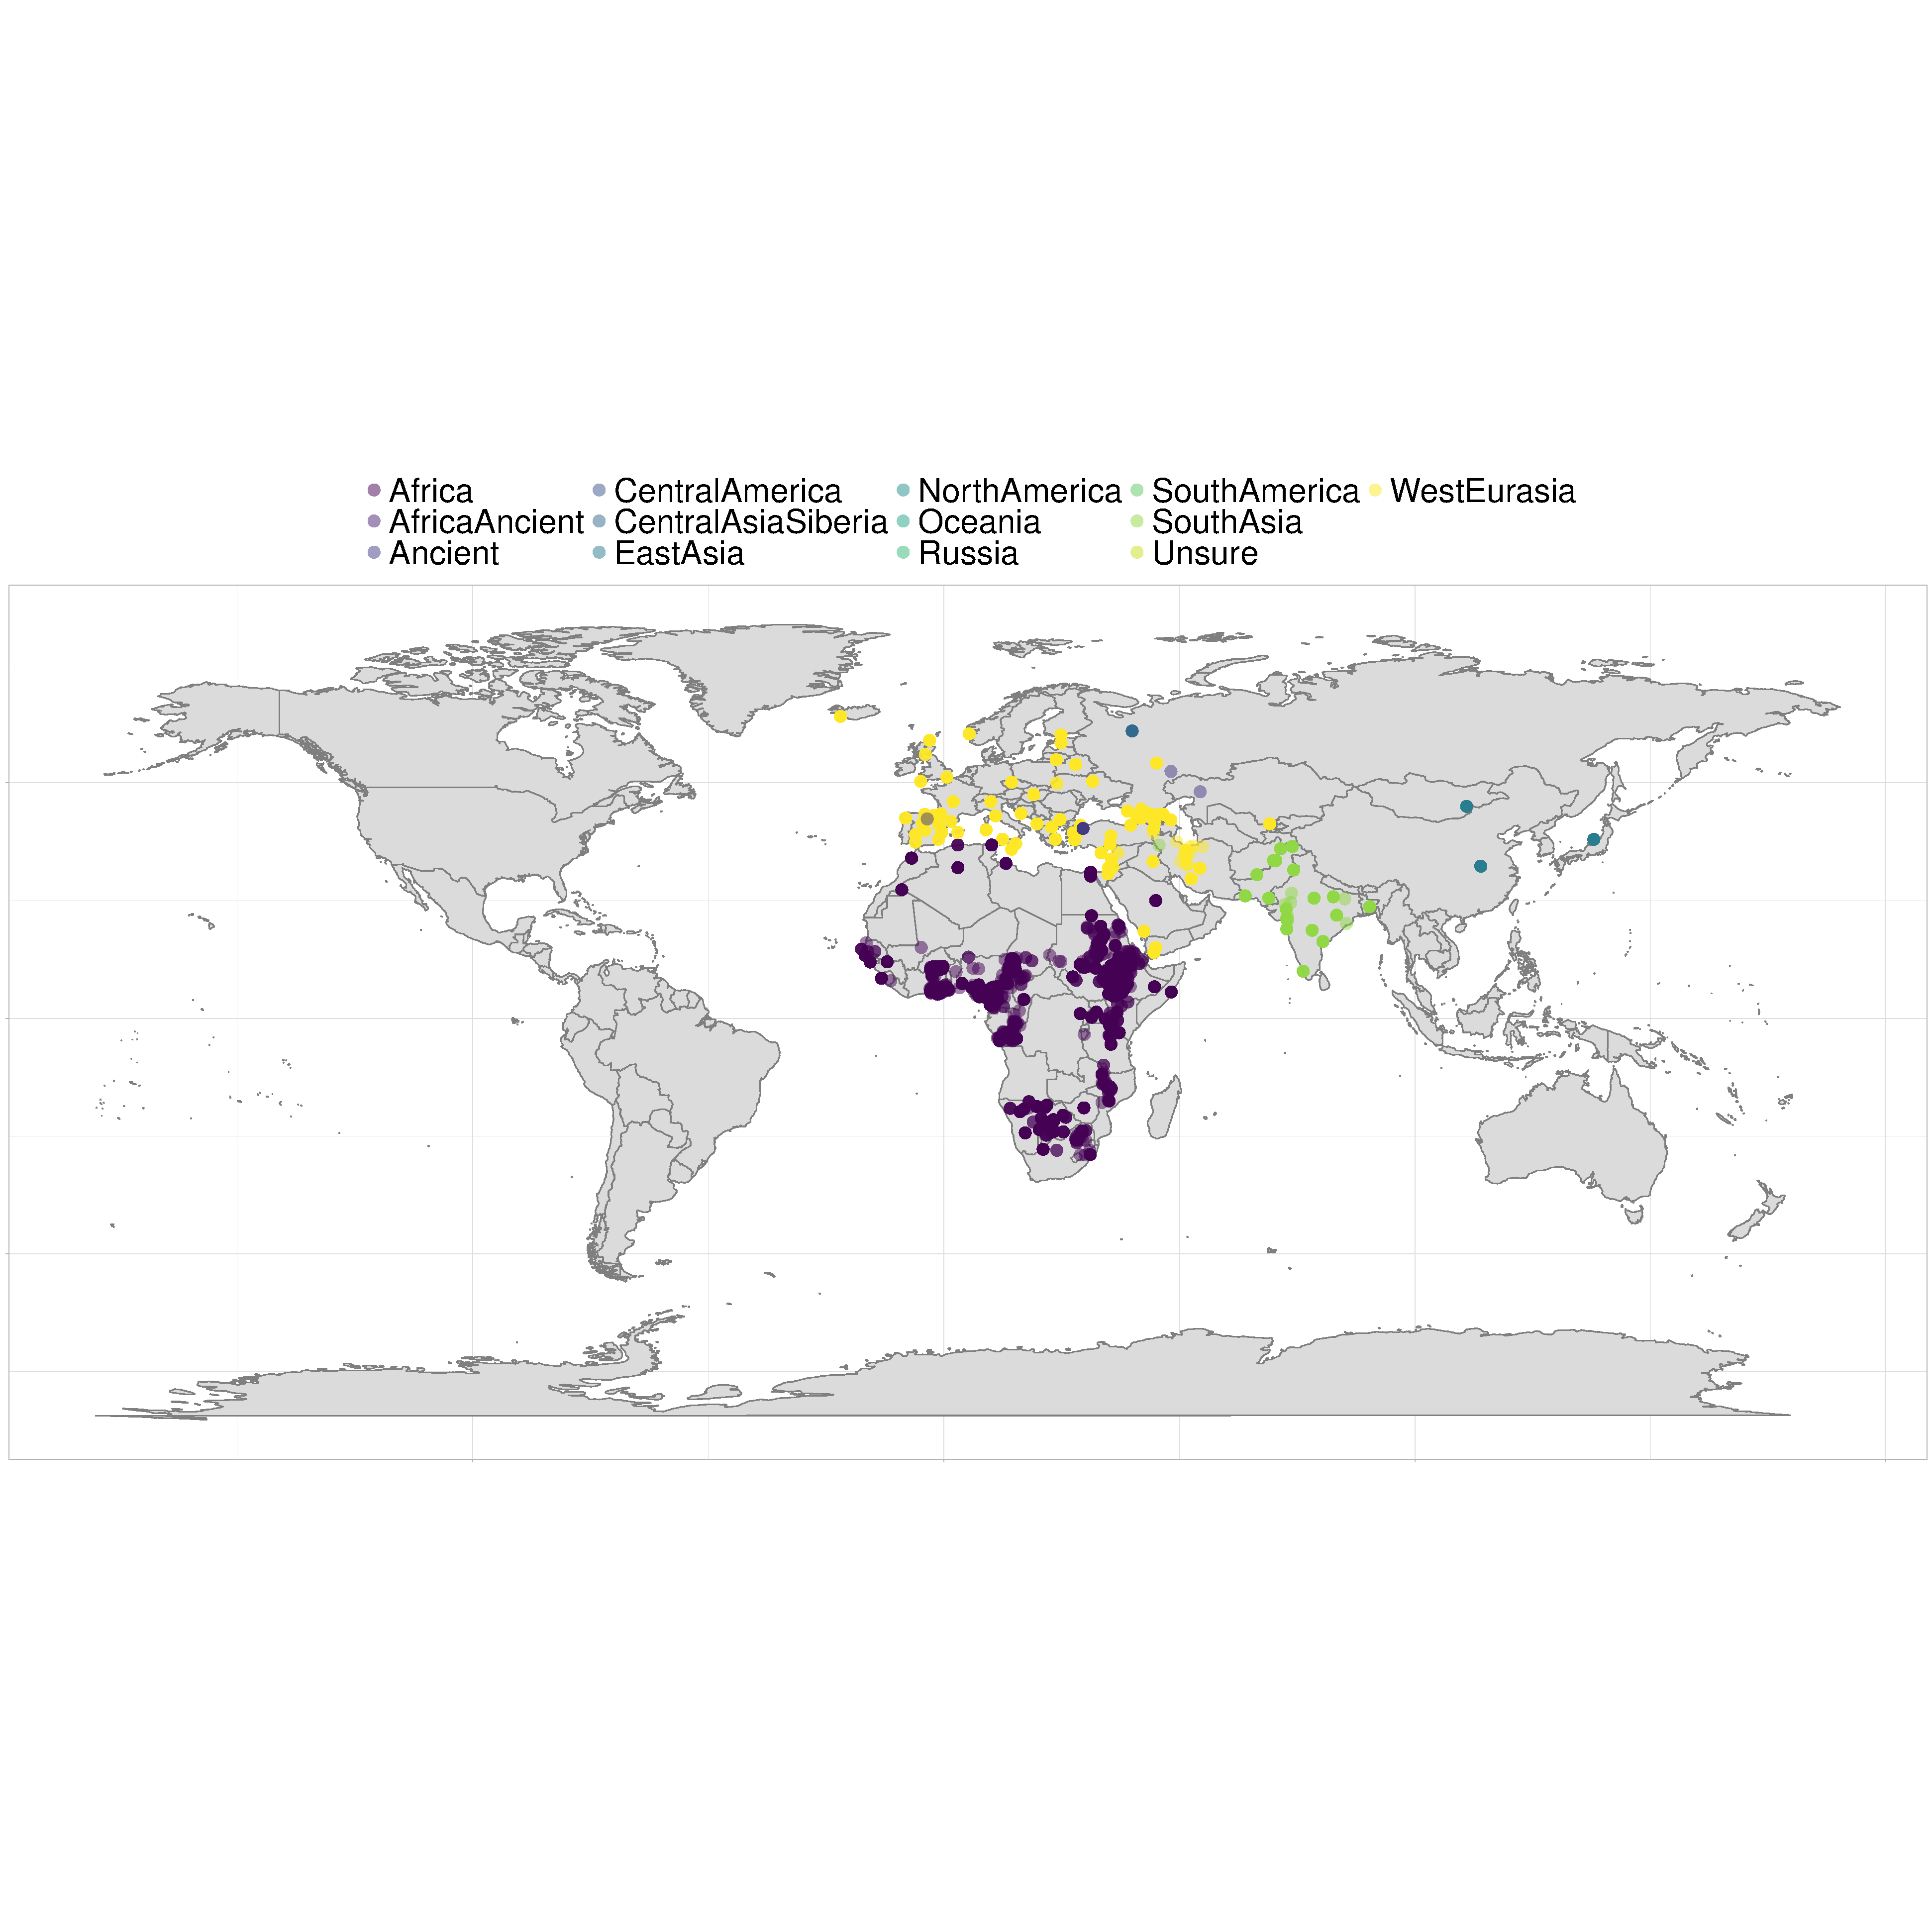
\includegraphics[width=1.0\textwidth]{../images/chapter3/HumanOriginsMap.pdf}
	    \caption{Map of Human Origins populations.}
	    \label{fig:HumanOriginsMap}
\end{sidewaysfigure}

\subsection{Data merge - non-imputed data and Human Origins}

I used \texttt{bcftools --merge} to merge 5,998 reference Human Origins dataset individuals with 8,476 UK Biobank participants that had $\geq$50\% African ancestry, using the gt-conform utility from Beagle (\url{https://faculty.washington.edu/browning/conform-gt.html}) to remove any inconsistent positions. This dataset contained 65,749 non-imputed SNPs that overlap between the Human Origins and UK Biobank arrays. I phased this dataset with shapeit4 \cite{delaneau2018integrative} using \texttt{--pbwt-depth 8}, the b37 genetic map and all other parameters set as default.  

\subsection{Data preparation - imputed data}

I similarly merged the imputed UK Biobank data with the Human Origins reference dataset at 525,566 SNPs that were genotyped in Human Origins, and phased this dataset with shapeit4, using the same settings as for the non-imputed data.

\subsection{ChromoPainter}

For both of the imputed and non-imputed datasets, I used ChromoPainter to infer the proportion of genome-wide DNA that each UK Biobank and Human Origins reference individual matches to individuals from each Human Origins reference population. 

An alternative option to using ChromoPainter would be to use PBWT (positional Burrows-Wheeler transform) paint (\url{https://github.com/richarddurbin/pbwt/blob/master/pbwtPaint.c}), a fast approximation to ChromoPainter which provides approximately the same output and is scalable to large sample sizes \cite{byrne2020dutch}. However, it is not possible to provide a reference panel and each haplotype must be compared to all others in turn. This would be much less efficient and would not allow me to take full advantage of the Human Origins dataset. 

\subsection{SOURCEFIND}

I estimated ancestry proportions for each of the selected U.K. Biobank individuals using SOURCEFINDv2 \cite{Chacon-Duque2018}. I used the combined painting from the section above. I analysed each U.K. Biobank individual with more than 50\% African ancestry separately, using all Human Origins populations as surrogates. I left all parameters as default. 

\subsection{Imputation bias test} \label{sec:ImputationBiasTest}

The imputed U.K. Biobank dataset was imputed using a reference panel containing the Haplotype Reference Consortium. Whilst this reference panel contains many European populations, it contains relatively few from Africa. Imputing variants in non-European individuals using a reference panel that is primarily composed of European individuals may leadf to biased or inaccurate imputation \cite{huang2011haplotype}. Given I am particularly interested in analysing individuals with recent African ancestry in the U.K. Biobank, it is important to determine whether this is the case.  

An obvious way to test this would be to compare a painting on the \textbf{U.K. Biobank} individuals using datasets comprised of a majority imputed and non-imputed SNPs. However, this is not possible; whilst the dataset contains country of birth (non-UK), the samples in the U.K. Biobank dataset do not have any associated population or ethnic group labels beyond broad self-identified categories. Accordingly, it would not be possible to mask their ethnic group and attempt to guess it using only the genetic data, an approach which I use for the Human Origins data in this chapter.

Therefore, I used the Human Origins dataset, where I could control whether or not SNPs are imputed and mask population labels. I submitted the full Human Origins reference dataset (5998 individuals and 560,420 SNPs) to the Sanger Imputation Server (\url{https://imputation.sanger.ac.U.K./}), which uses the full Haplotype Reference Consortium (HRC) as a reference panel for imputation. 
I subsetted the imputed Human Origins dataset down to SNPs present in the U.K. Biobank array, leaving 727,325 positions present in the imputed Human Origins dataset and then randomly removed SNPs until 500,000 remained. Although the number of SNPs still differ, my previous research in Chapter 2 shows that increasing the number of SNPs beyond 400,000 does not affect the ability to correctly assign individuals to populations (Appendix section \ref{sec:SNP_Count_Assignment_DevCorn}). I phased the imputed and non-imputed datasets separately using shapeit4 at default settings. 

To  therefore determine whether using the imputed or the 70,000 SNP Human Origins dataset is better in this scenario, I performed a painting using (i) the full 560,442 genotyped SNPs, (ii) 64,762 genotyped SNPs overlapping UK Biobank, and (iii) 500,000 SNPs that include the 70,000 genotyped SNPs and 430,000 SNPs imputed using the HRC reference. I performed painting (ii) in both linked and unlinked mode to determine whether there is haplotype information using 70,000 SNPs.

For each of the three datasets described above, I selected all ethnic groups from Nigeria, Cameroon and Ghana which had five or more individuals (n=51 populations, n=1203 individuals) and split each population randomly in half, into `donors' and `recipients'. I painted all recipient populations (n=51) using all donor populations (n=51) using a leave-one-out approach (motivation for this approach given in Appendix section \label{sec:leave_one_out}). I tested the information content of each painting by counting how often individuals copy more from individuals in their own populations than individuals from other populations. I also counted the number of times a population had the lowest TVD (motivation and description of TVD given in appendix section \ref{sec:appendixTVD}) with its own population (Table \ref{table:TVD_copying}).

\section{Results}

\subsection{4\% of U.K. Biobank individuals have at least 50\% non-European ancestry}

Performing ChromoPainter analysis on the 488,378 individuals in the U.K. Biobank would be computationally unfeasible; therefore I first performed supervised ADMIXTURE on all U.K. Biobank individuals. In order to identify individuals with at least 50\% African ancestry, I set $K=4$ supervision clusters that were defined using European (CEU), Gujarati, Han Chinese and Yoruban reference individuals from the 1000 genomes dataset. I then carried forward individuals with more than 50\% ancestry from Yoruba to later ChromoPainter analyses.

In total, there were 8476, 2653, 9171 individuals with at least 50\% ancestry most closely related to either Yoruba, Han Chinese and Gujarati reference populations respectively, corresponding to 4.16\% of the total U.K. Biobank individuals. Although I use these population labels for convenience, I note that an individual with e.g. 50\% `Han Chinese' ancestry does not necessarily derive 50\% of their ancestry from the Han Chinese population, but that 50\% of their ancestry most closely matches Han China relative to the other reference populations. Thus, a Japanese individual may be modelled as 100\% Han Chinese whilst not being Han Chinese in an ethnic sense. Similarly, for brevity, I will refer to individuals who have more than 50\% of their ancestry from Yoruba as being `African' Biobank individuals, whilst acknowledging that `African' as a broad label encompasses a large diversity of ancestries and ethnicities.  

I validated the ADMIXTURE results to ensure that there was not any mixing of sample labels and that enough ADMIXTURE EM iterations had been performed. To do this, I selected all individuals who self-identified as being either "Caribbean", "African" or "Black or Black British" (n=7,527) and plotted the distribution of ADMIXTURE ancestry proportions, under the assumption that these individuals should contain more African than other kinds of ancestry. On average this was the case, with the mean proportion of African ancestry among these individuals being 0.88 (Fig. \ref{fig:African_Inds_proportions_ADMIXTURE}), compared to 11 \% British, 0.22\% Han Chinese and 0.19\% Gujarati.

However, there was substantial variation in the ancestry proportions for those who self-identified as being either "Caribbean", "African" or "Black or Black British". Proportions of Yoruban and British ancestry ranged from 0 to 1, Han Chinese from 0 to 0.53 and Gujarati from 0 to 0.759, reflecting the diverse array of genetic ancestries that can fall under a given ethnic label. This follows from previous research which has shown self-reported ethnicity can be an unreliable proxy for genetic ancestry \cite{shraga2017evaluating, LouwersSelfReportedEthnicity2014}. This suggests that relying on self-reported ethnicity may yield variable results when e.g. used as a covariate in a GWAS. For example, there were 48 people who self identified as being either "Caribbean", "African" or "Black or Black British", but had less than 1\% African ancestry.

\begin{figure}[htp]
    \centering
    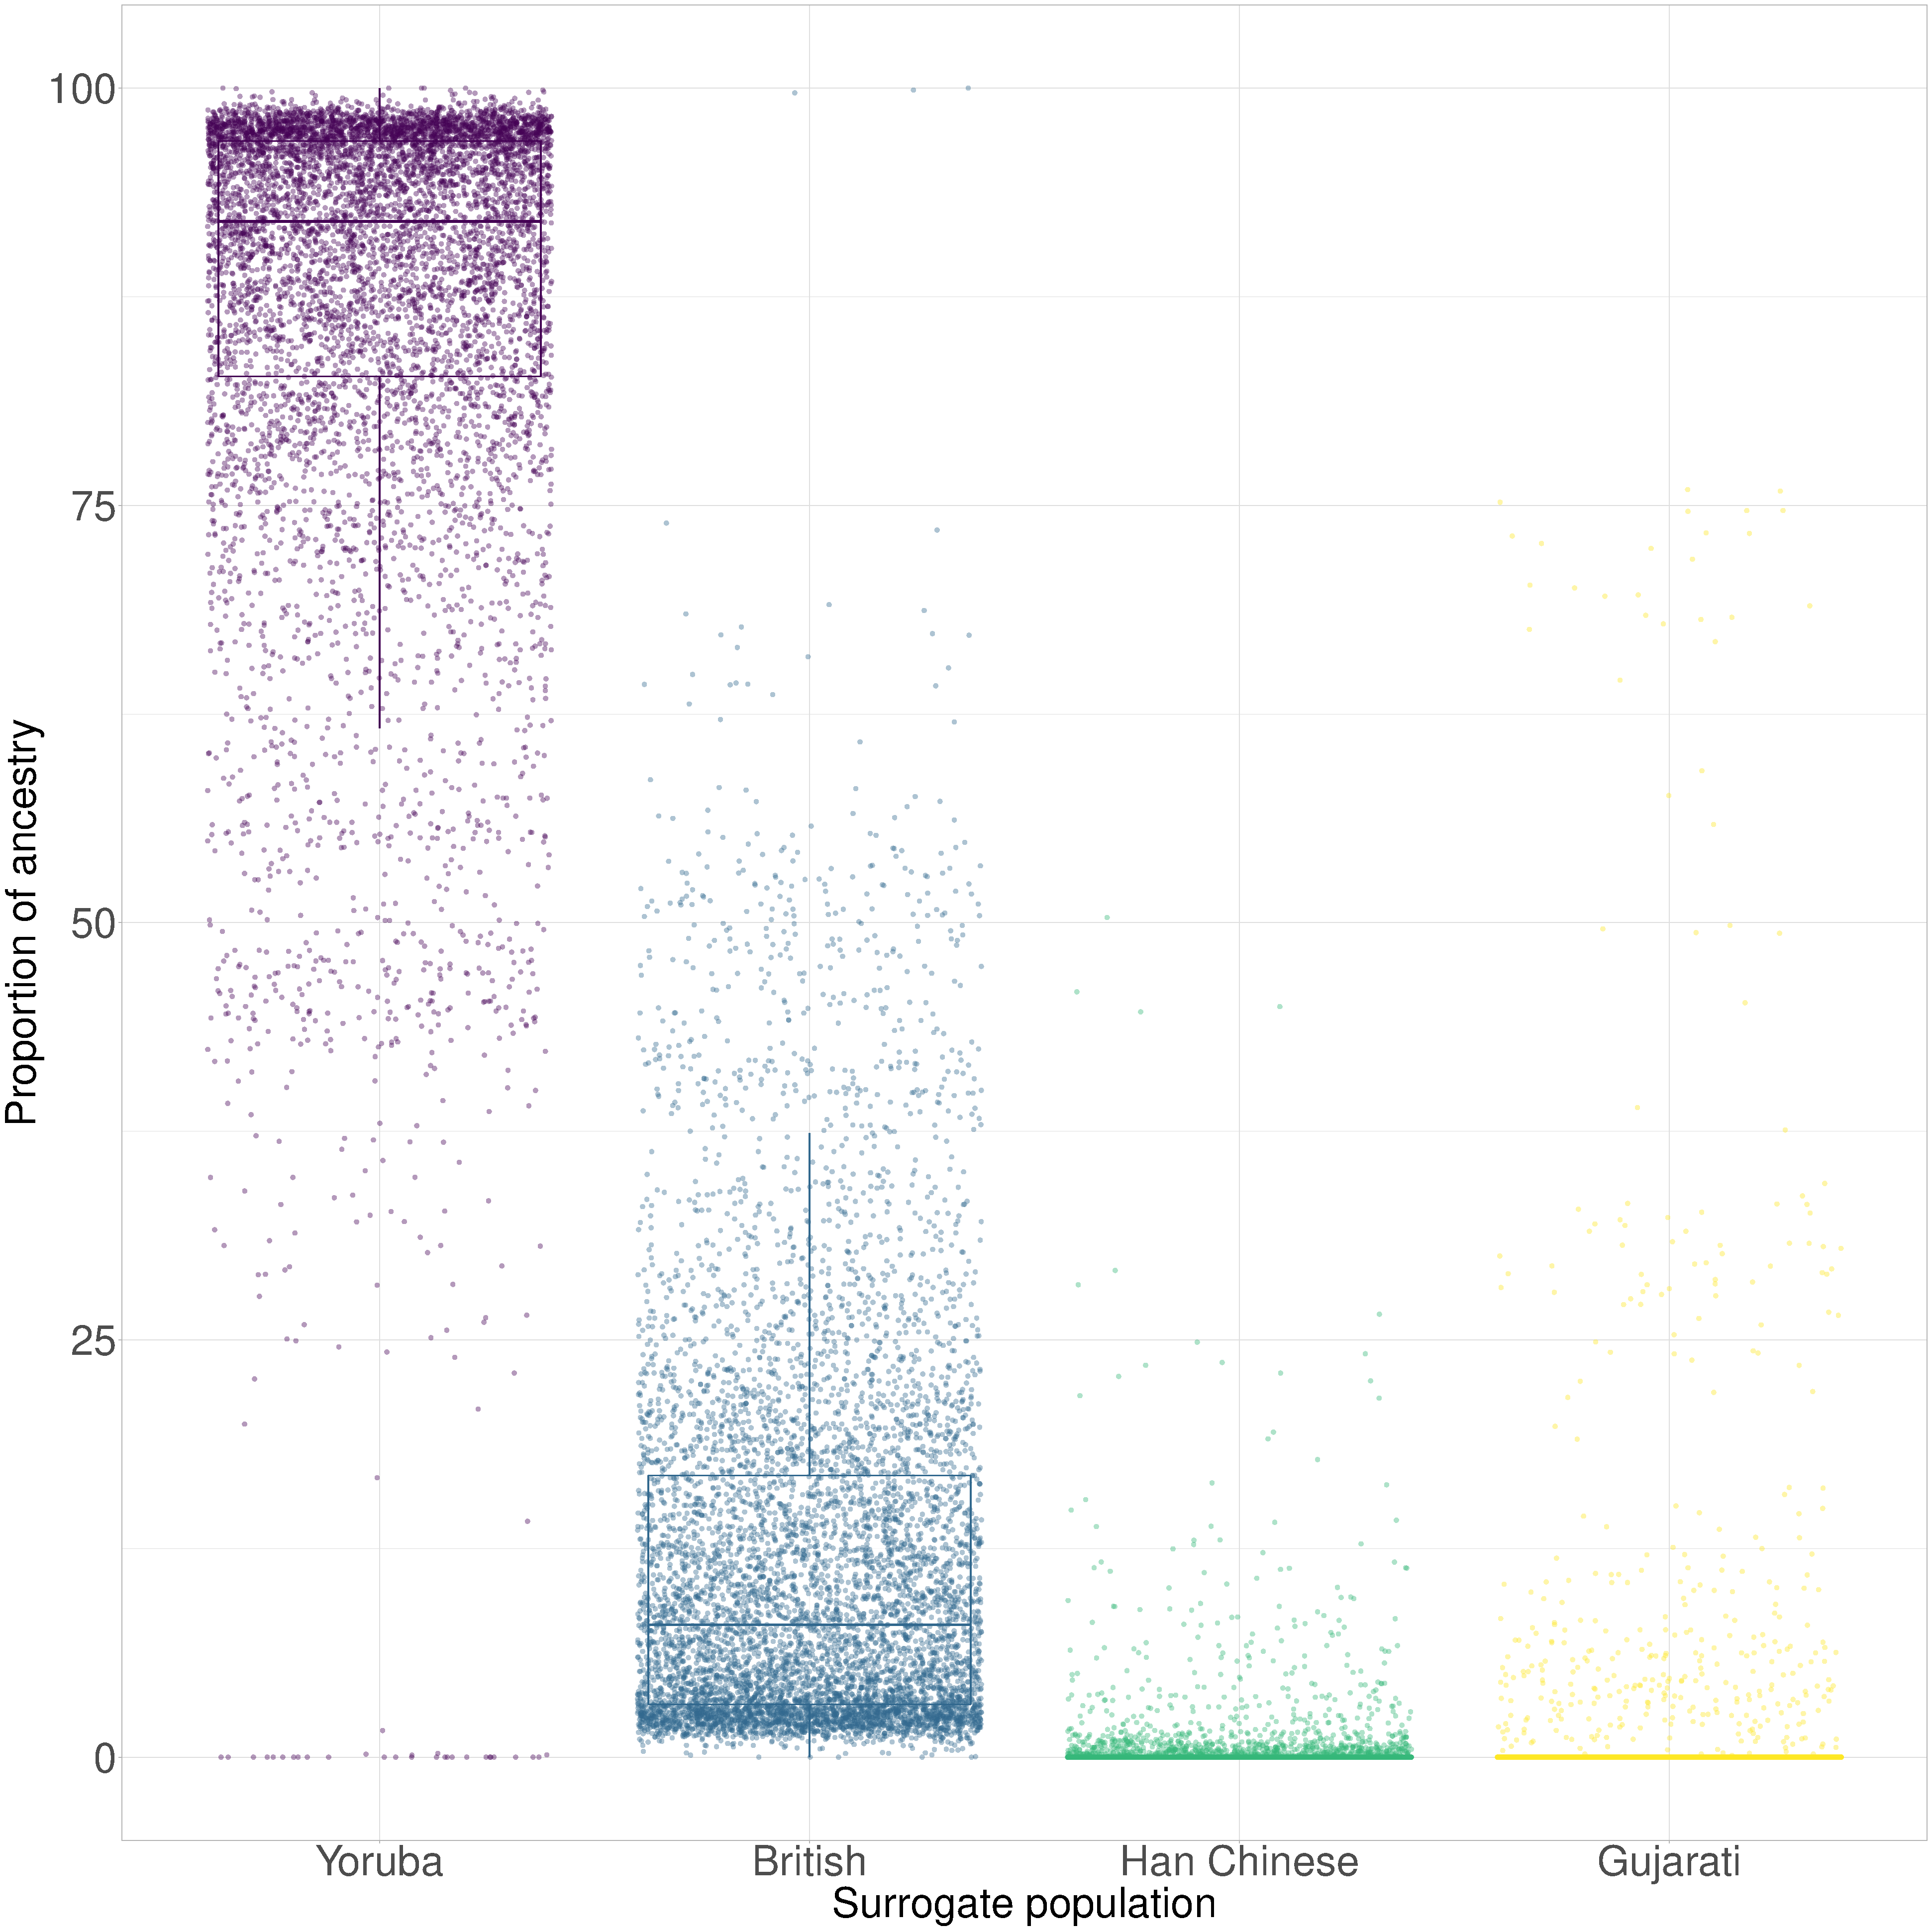
\includegraphics[width=1.0\textwidth]{../images/chapter3/African_Inds_proportions.pdf}
    \caption{Ancestry proportions inferred from supervised ADMIXTURE run (k=4) for all individuals who self identified as being either "Caribbean", "African" or "Black or Black British". Points within each column are given random jitter to improve visual clarity.}
    \label{fig:African_Inds_proportions_ADMIXTURE}
\end{figure}

\subsection{To impute or not?}

In order to use the Human Origins dataset as a reference in ChromoPainter analysis to ancestry in U.K. Biobank individuals, the datasets must be merged. The overlap of SNPs genotyped in each dataset is only 70,776 SNPS, or an average of $\approx$1 SNP per 40Kb. Given linkage disequilibrium (e.g.\ as measured by Pearson's correlation) between pairs of SNPs decays to background levels by 100Kb within most populations \cite{bosch2009decay}, analysing 70,000 SNPs may substantially decrease any potential power gains from modeling haplotypes to detect fine-scale differences between populations. In contrast, the imputed U.K. Biobank dataset has 535,544 SNPs in total, all of which are genotyped in the Human Origins reference dataset and 87.7\% of which are imputed in UK Biobank individuals. While this may boost power over using only 70,000 SNPs, including a high percentage of imputed SNPs may bias ancestry inference. Therefore, I needed to determine a) whether there is a loss of power when 70,000 SNPs relative to the a full 500,000 SNP dataset and b) whether there is bias when using a dataset which contains a majority of imputed SNPs.  

To answer these questions, I returned to the imputed and unimputed Human Origins datasets I describe in Section \ref{sec:ImputationBiasTest}. Recall here I reduced the Human Origins dataset to 70K SNPs and then imputed to approximately 500,000 SNPs using HRC and therefore determine whether using the imputed or the 70,000 SNP Human Origins dataset is better in this scenario, I performed a painting using (i) the full 560,442 genotyped SNPs, (ii) only the 64,762 genotyped SNPs overlapping UK Biobank, and (iii) 500,000 SNPs that include the 64.47K genotyped SNPs and 430,000 SNPs imputed using the HRC reference. I performed painting (ii) in both linked and unlinked mode to determine whether there is any haplotype information using 70,000 SNPs.

It is worth noting that, because of the specific SNP ascertainment strategies used, a sizeable fraction of Human Origins SNPs have a very low frequency; 7 SNPs were invariant, 104,442 had a minor-allele frequency of less than 0.05, 35,061 of less than 0.01 and 2,891 less than 0.001 (Fig. \ref{fig:MAF_HIST_imputed}).

For each of the three datasets described above, I selected all ethnic groups from Nigeria, Cameroon and Ghana which had five or more individuals (n=51 populations, n=1203 individuals) and split each population randomly in half, into `donors' and `recipients'. I painted all recipient populations (n=51) using all donor populations (n=51) using a leave-one-out approach (description and motivation of this approach given in Appendix section \ref{sec:leave_one_out}). I only considered populations of five individuals or more because any fewer individuals would likely result in very weak power to assign individuals to that population. I tested the information content of each painting by counting how often individuals copy more from individuals in their own populations than individuals from other populations. I also counted the number of times a population had the lowest TVD (motivation and description of TVD given in Appendix section \ref{sec:appendixTVD}) with the mean copyvector of all other individuals in its own population (Table \ref{table:TVD_copying}).

Populations in the 70,000 non-imputed painting matched more to and had a lower $TVD$ with their own mean population copyvector than the 500,000 non-imputed painting. These results suggest that, in the context of performing ChromoPainter analysis to assign African individuals to sub-continental ethnic groups, there is no clear benefit to using more than 70,000 SNPs. Whilst it may seem counter-intuitive that there is more power using a smaller number of SNPS, this is broadly consistent with my previous findings in Chapter 2, which showed that metrics of painting information plateau (Fig. \ref{fig:Devon_Cornwall_TVD_reduced_assignment}) (i.e.\ there is no clear benefit to using more than 50,000 SNPs in terms of assigning individuals to a population). This is reassuring and suggests there is no loss of power when using the 70,000 SNP set. It is worth noting that there may be advantages to using a higher number of SNPs in other contexts; for instance, when attempting to identify which population genomic segments may have originated from in GLOBETROTTER admixture analysis.

This data also shows that there is a fairly dramatic loss of power when using imputed data relative to non-imputed data, as over 3x the number of populations had a lower TVD with their own population when using imputed compared to non-imputed data.

\begin{table}
\centering
\small
\begin{tabular}{l|l|l}
\toprule
painting & TVD & copying\\
\midrule
70K (linked) & 44\% & 24\%\\
70K (unlinked) & 20\% & 17\%\\
imputed (linked) & 14\% & 14\%\\
full (linked) & 38\% & 23\%\\
\bottomrule
\end{tabular}
\caption{Percentage of populations which had lowest TVD (TVD) or copied the most (copying) from their own population under different paintings. 70K linked used 70,000 SNPs in linked mode, 70K used 70,000 SNPs in unlinked mode, imputed used 430,000 imputed and 70,000 non-imputed SNPs in linked mode and full used 500,000 non-imputed SNPs in linked mode.}
\label{table:TVD_copying}
\end{table}

Given the above results suggested that imputing data results in a loss of information, I was interested in whether this constituted a `bias' towards certain populations. Reference-based imputation methods rely on identifying reference haplotypes which are closest to the target haplotypes. However, if the ethnic groups that the target individuals derive ancestry from are not present in the imputation reference panel, missing variants are imputed from populations in the reference panel which are most closely related to the target samples. In this case, two target populations may be imputed to appear more genetically similar to that reference population, reducing the differentiation between them (Fig \ref{fig:imputed_nonimputed_donation}). In theory, this artificial similarity would be propagated through to the ChromoPainter analysis. In particular, we would expect populations present in the reference panel to donate more to all other individuals than they would if no imputation had taken place.  

For example, in the case of the Haplotype Reference Consortium, the closest reference population to two African target samples from e.g. Cameroon may be the Yoruba from Nigeria, which is one of the few west African groups in the reference. These samples would appear more similar to the Yoruba ethnic group than if they had not been imputed. In a ChromoPainter analysis, the Yoruba donor population would donate more than than when using non-imputed SNPs.    

Comparing the imputed and non-imputed coancestry matrices revealed biases consistent with the above expectation. If the coancestry matrix columns are combined into populations, then the sum of each column gives the total length of genome that population contributes to all recipient individuals in the dataset. Therefore, comparing the column sums between the imputed and non-imputed matrices informs us about which populations contribute more when using imputed compared to non-imputed SNPs. Fig \ref{fig:imputed_excess_copying_pops} shows the amount of differential haplotype donation on a per-population basis, with populations highlighted based on their presence or absence in the 1000 genomes dataset. It is clear that populations present in the 1000 genomes are primarily clustered towards the right hand side, rather than randomly distributed across figure. This strongly suggests that imputation causes a bias towards those populations present in a reference panel. 

To formally test whether the ordering of populations was likely significantly different to the ordering expected under the null model of no impact of being present in the 1000 genomes dataset, I performed a non-parametric permutation test. If we order the populations based on their differential haplotype donation and assign a rank value to each population, we can calculate the sum, $S$ of the ranks values of all populations present in the 1000 genomes. If the 1000 genomes populations are clustered at the higher end of the ordering, we would expect the value of $S$ to be smaller than if the populations are randomly distributed across the ordering. I performed 100,000 replications of randomly ordering the population labels and calculating the value of $S$. Of the 100,000, 26 had $S$ greater than the true empirical value calculated from the data, showing the ordering of the populations is unlikely to be due to chance ($p=0.00026$). This permutation test was motivated by the Wilcoxon Rank Sum Test.  

\begin{sidewaysfigure}
	    \centering
	    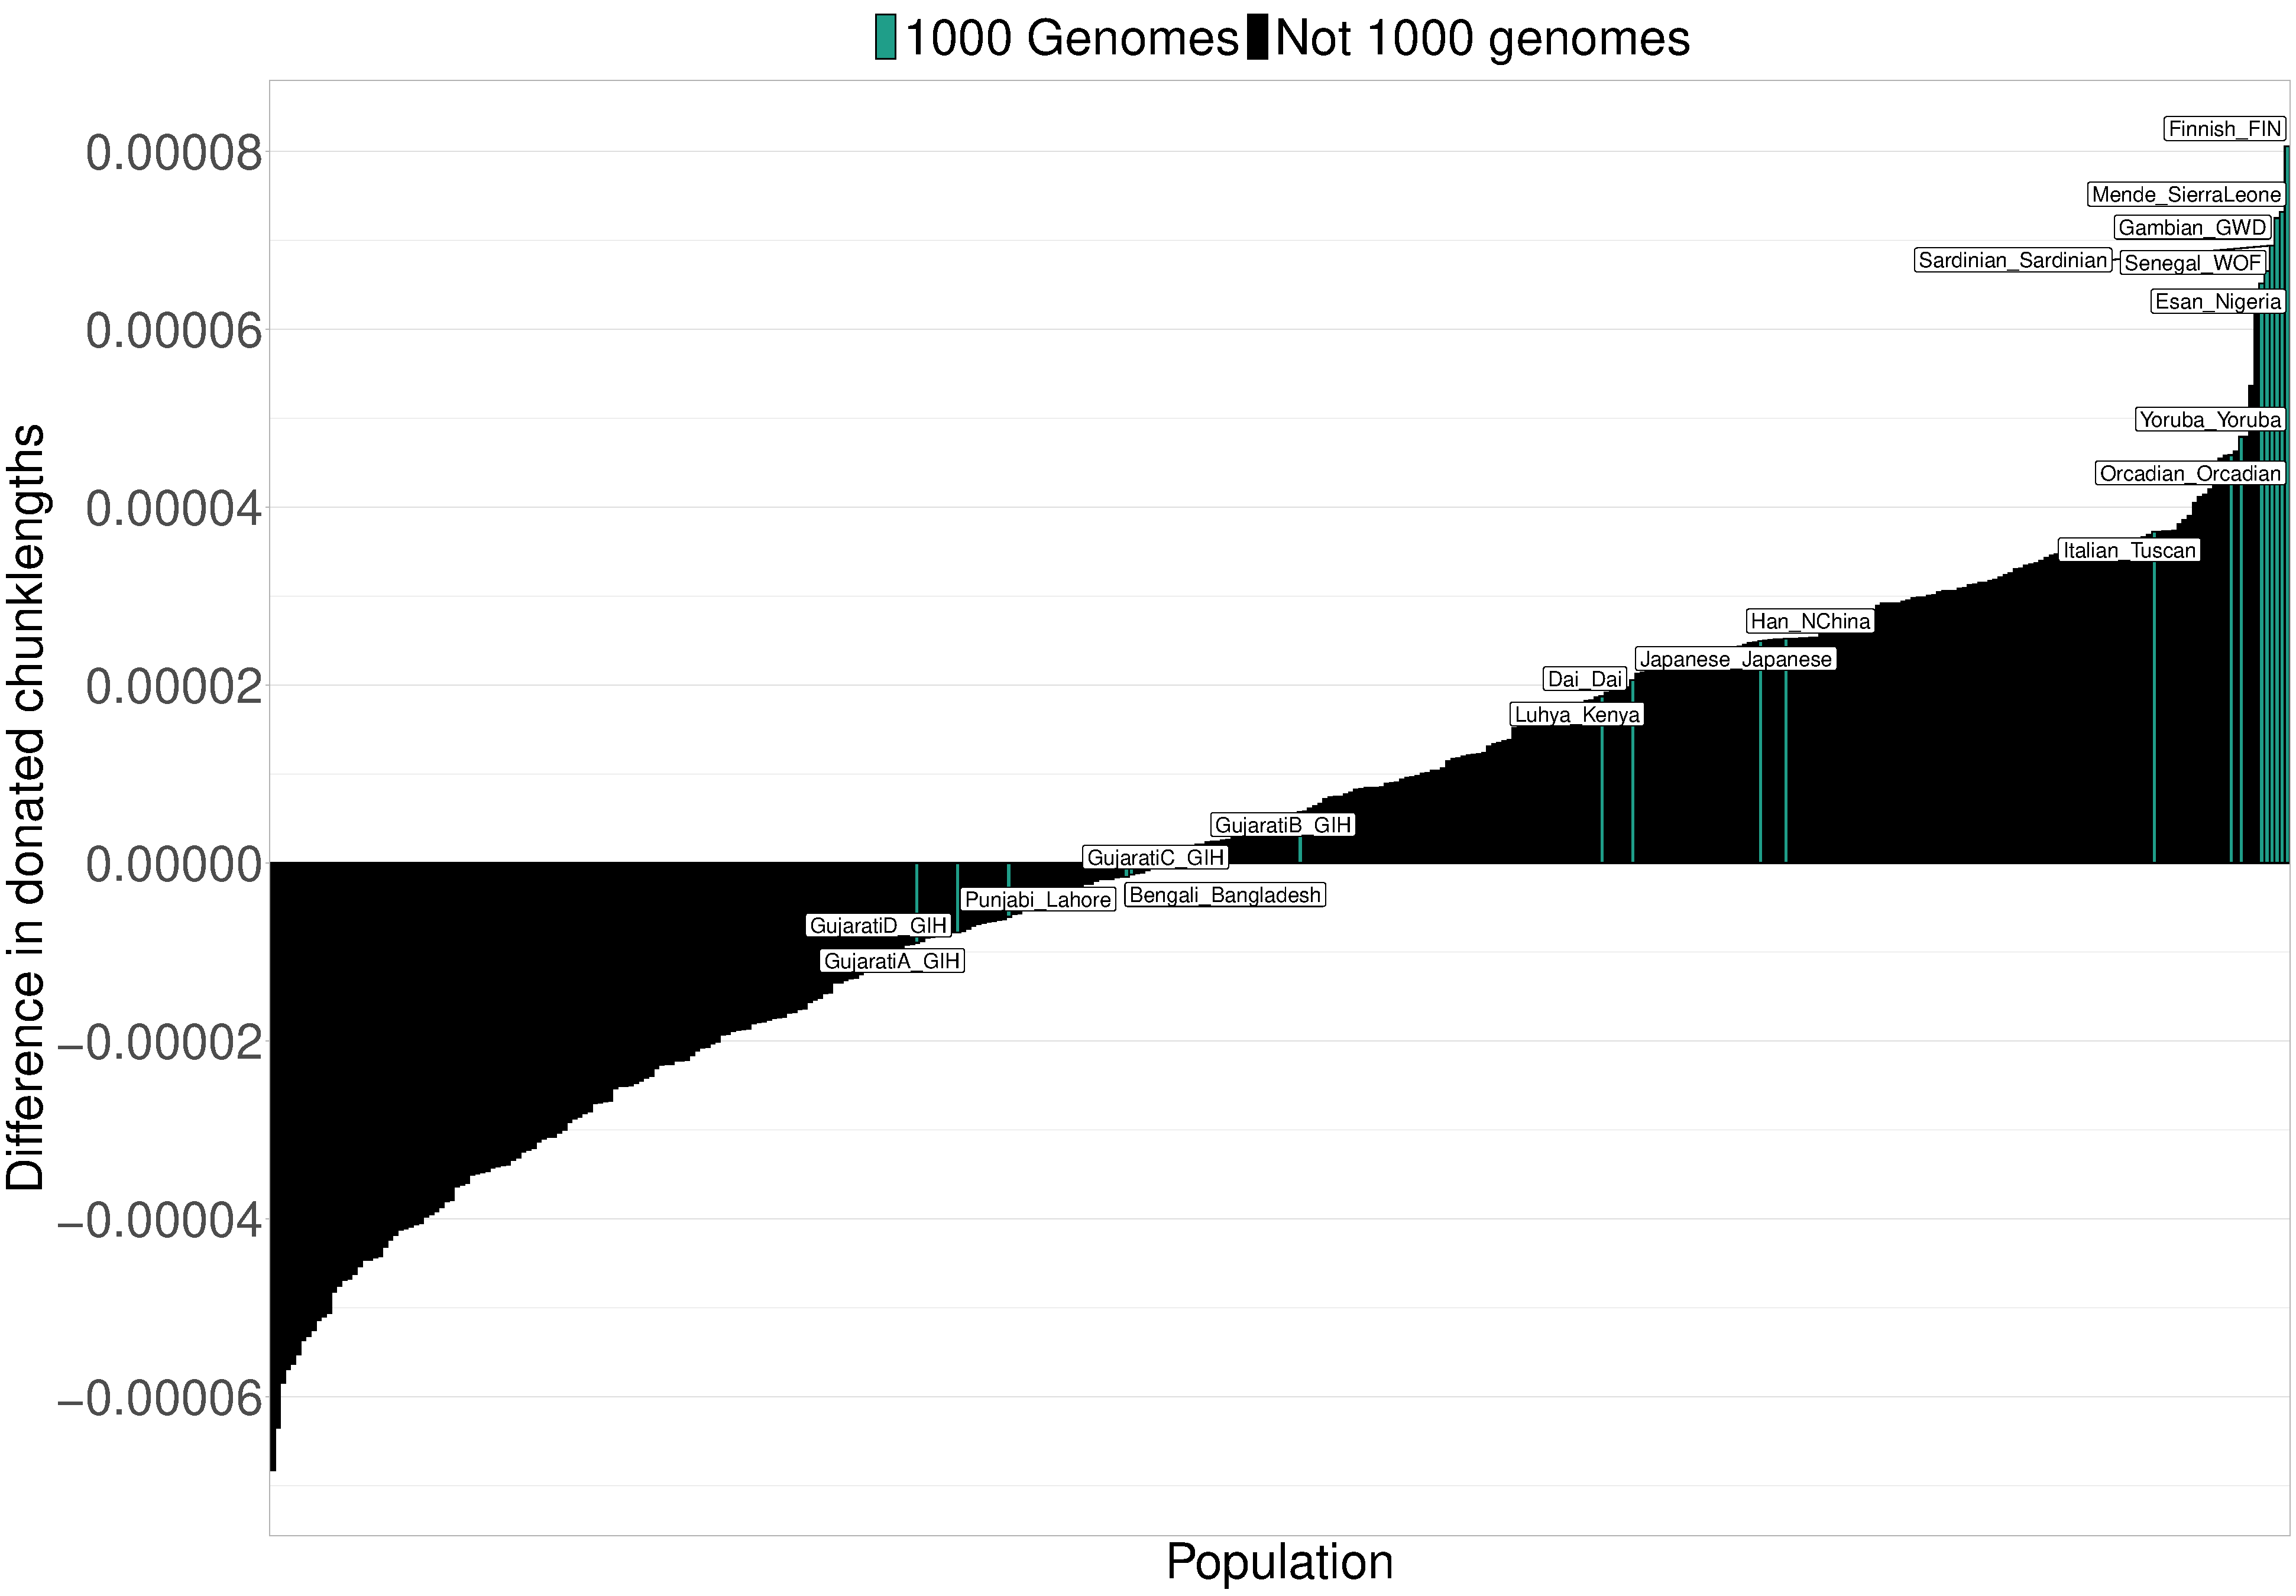
\includegraphics[width=1.0\textwidth]{../images/chapter3/imputed_excess_copying_pops.pdf}
	    \caption{Differences in the amount donated by populations when using imputed and non-imputed data. Each vertical bar corresponds to a single population (N=395), with the height of the bar corresponding to the difference in haplotype donation, with positive values indicating increased donation and negative values indicating reduced donation. Bars coloured in green are also present in the 1000 genomes imputation panel and black bars are not present in the 1000 genomes.}
	    \label{fig:imputed_excess_copying_pops}
\end{sidewaysfigure}

Put together, these results suggest that using imputed data would introduce a level of bias and loss of information when trying to accurately infer sub-continental ancestry of African individuals that may obscure the true pattern of African ancestry in U.K. Biobank participants. In particular, we would expect an additional 10\% of individuals to be misclassified to the correct ethnic group when using imputed compared to non-imputed data.

Therefore, with the exception of exercises comparing the imputed and non-imputed data, in all later analysis, I chose to use the approximately 70,000 non-imputed SNPs which overlap between the Human Origins and U.K. Biobank datasets. 

\subsection{African ancestry in the U.K. Biobank samples is concentrated in Ghana and Nigeria}

Using approximately 70,000 directly genotyped SNPS, I painted all U.K. Biobank individuals with at least 50\% African ancestry (n=8475) using all Human Origins individuals as donors (n=5,577).

Principal component analysis on the resulting chunkcounts coancestry matrix reveals the general structure of the selected individuals, alongside the reference populations (Fig. \ref{fig:PCA_chunklengths_HumanOrigins_U.K.Biobank}). Three clines are present; one of similarity to Southern African populations typified by the Zulu ethnic group from South Africa, one of similarity to West African populations such as Yoruba and Cameroon\_Dii, and the last to East African populations such as those from Ethiopia. The majority of U.K. Biobank individuals are positioned near West African populations; in particular between Yoruba and Cameroon\_Arabe. The presence of a broad cluster of West African individuals is consistent with prior expectations that West African ancestry should be prevalent in a sample of British individuals, due to the history of migration from this region \cite{banton1953recent}. A second cluster of UK Biobank individuals is located along the Southern African cline, close to the Bantu\_SA label. 

\begin{figure}[htp]
    \centering
    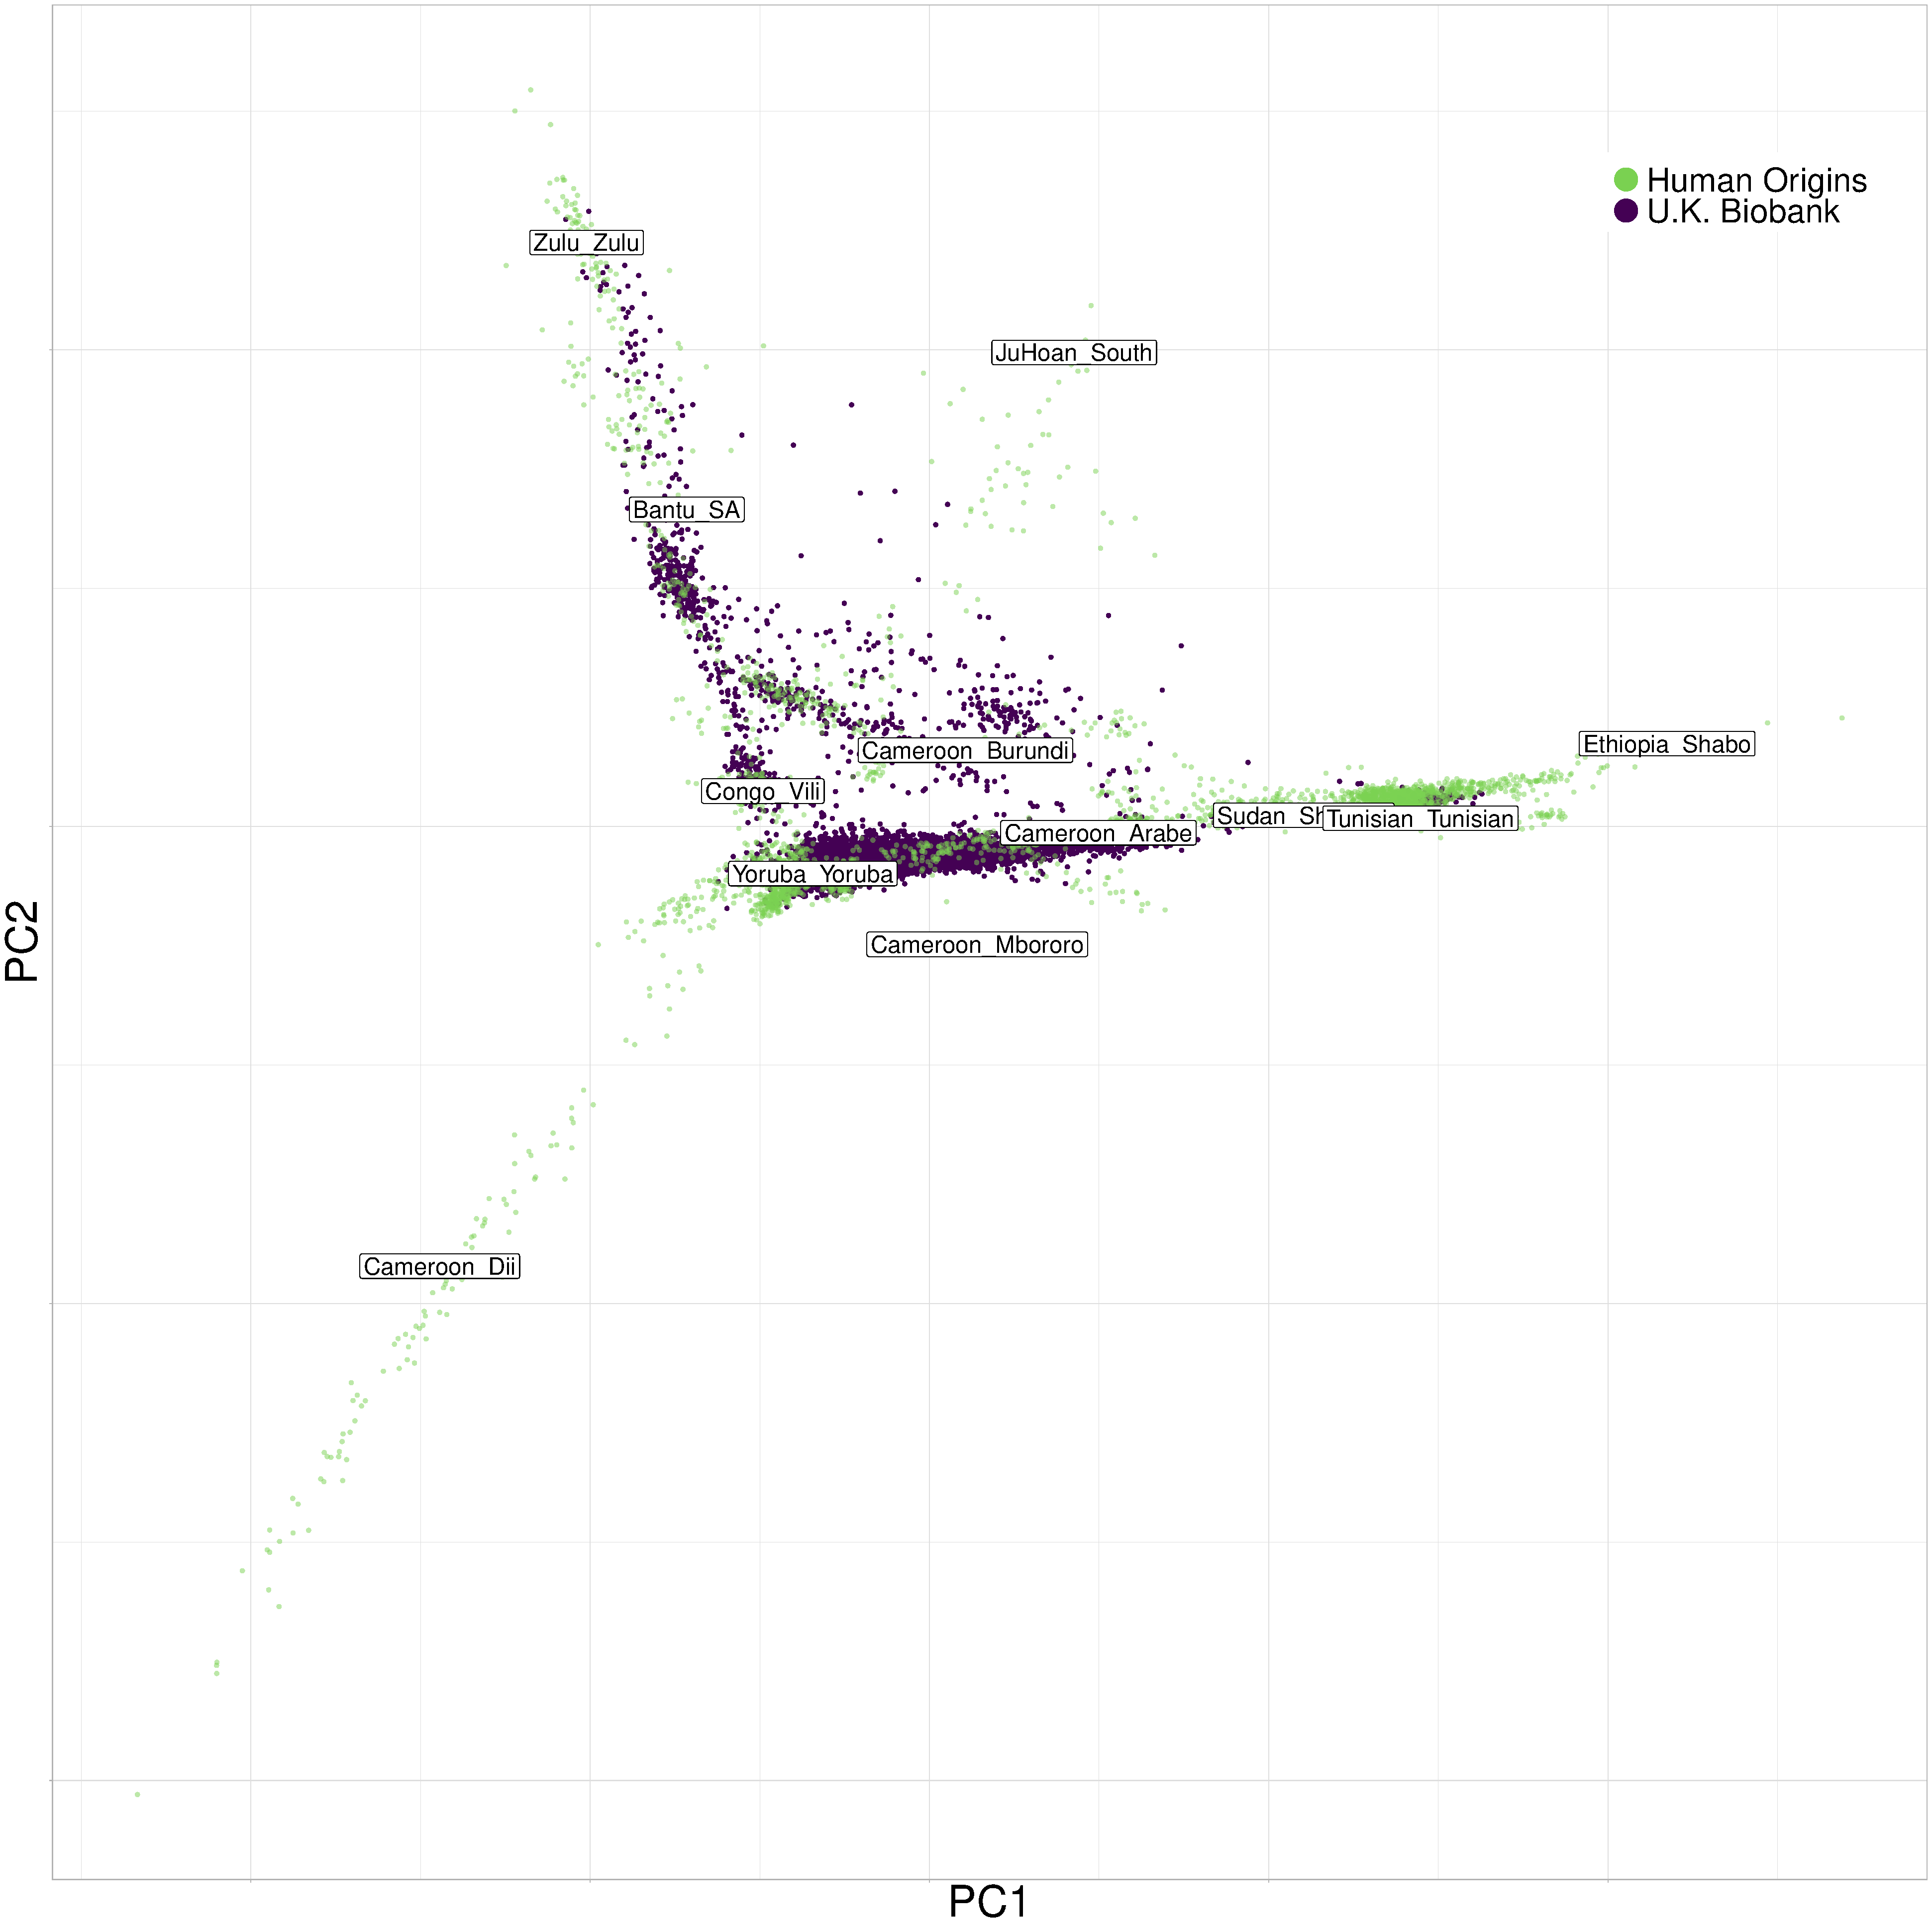
\includegraphics[width=1.0\textwidth]{../images/chapter3/ChromoPainter_PCA_UKB_HO.pdf}
    \caption{Principle component analysis of chunklengths matrix for U.K. Biobank individuals with $\geq$50\% inferred recent African ancestry and human origins array. Individuals are coloured dependent on whether they are U.K. Biobank (green) or Human Origins (purple) samples. Labels indicate mean principle component coordinates for individuals in that population. A random sample of populations were chosen to have labels to prevent the figure from being too cluttered.}
    \label{fig:PCA_chunklengths_HumanOrigins_U.K.Biobank}
\end{figure}

Aggregating the columns of the coancestry matrix by reference population and taking the sum of each column gives the total length of genome for which a U.K. Biobank individual shares recent ancestry with individuals from that donor population. This can be visualised on a map, where each point represents a reference population and the colour corresponds to the total amount that reference population contributes towards the ancestry of all retained U.K. Biobank individuals (Fig. \ref{fig:haplotype_sharing_map_zoomed_II}). Higher values correspond to more ancestry from that population in the U.K. Biobank sample. However, it should be noted that raw ChromoPainter output can be influenced strongly by sample size and so the values shown in Fig. \ref{fig:haplotype_sharing_map_zoomed_II} should not be taken literally as an exact reflection of the ancestry distribution.

\begin{figure}[htp]
    \centering
    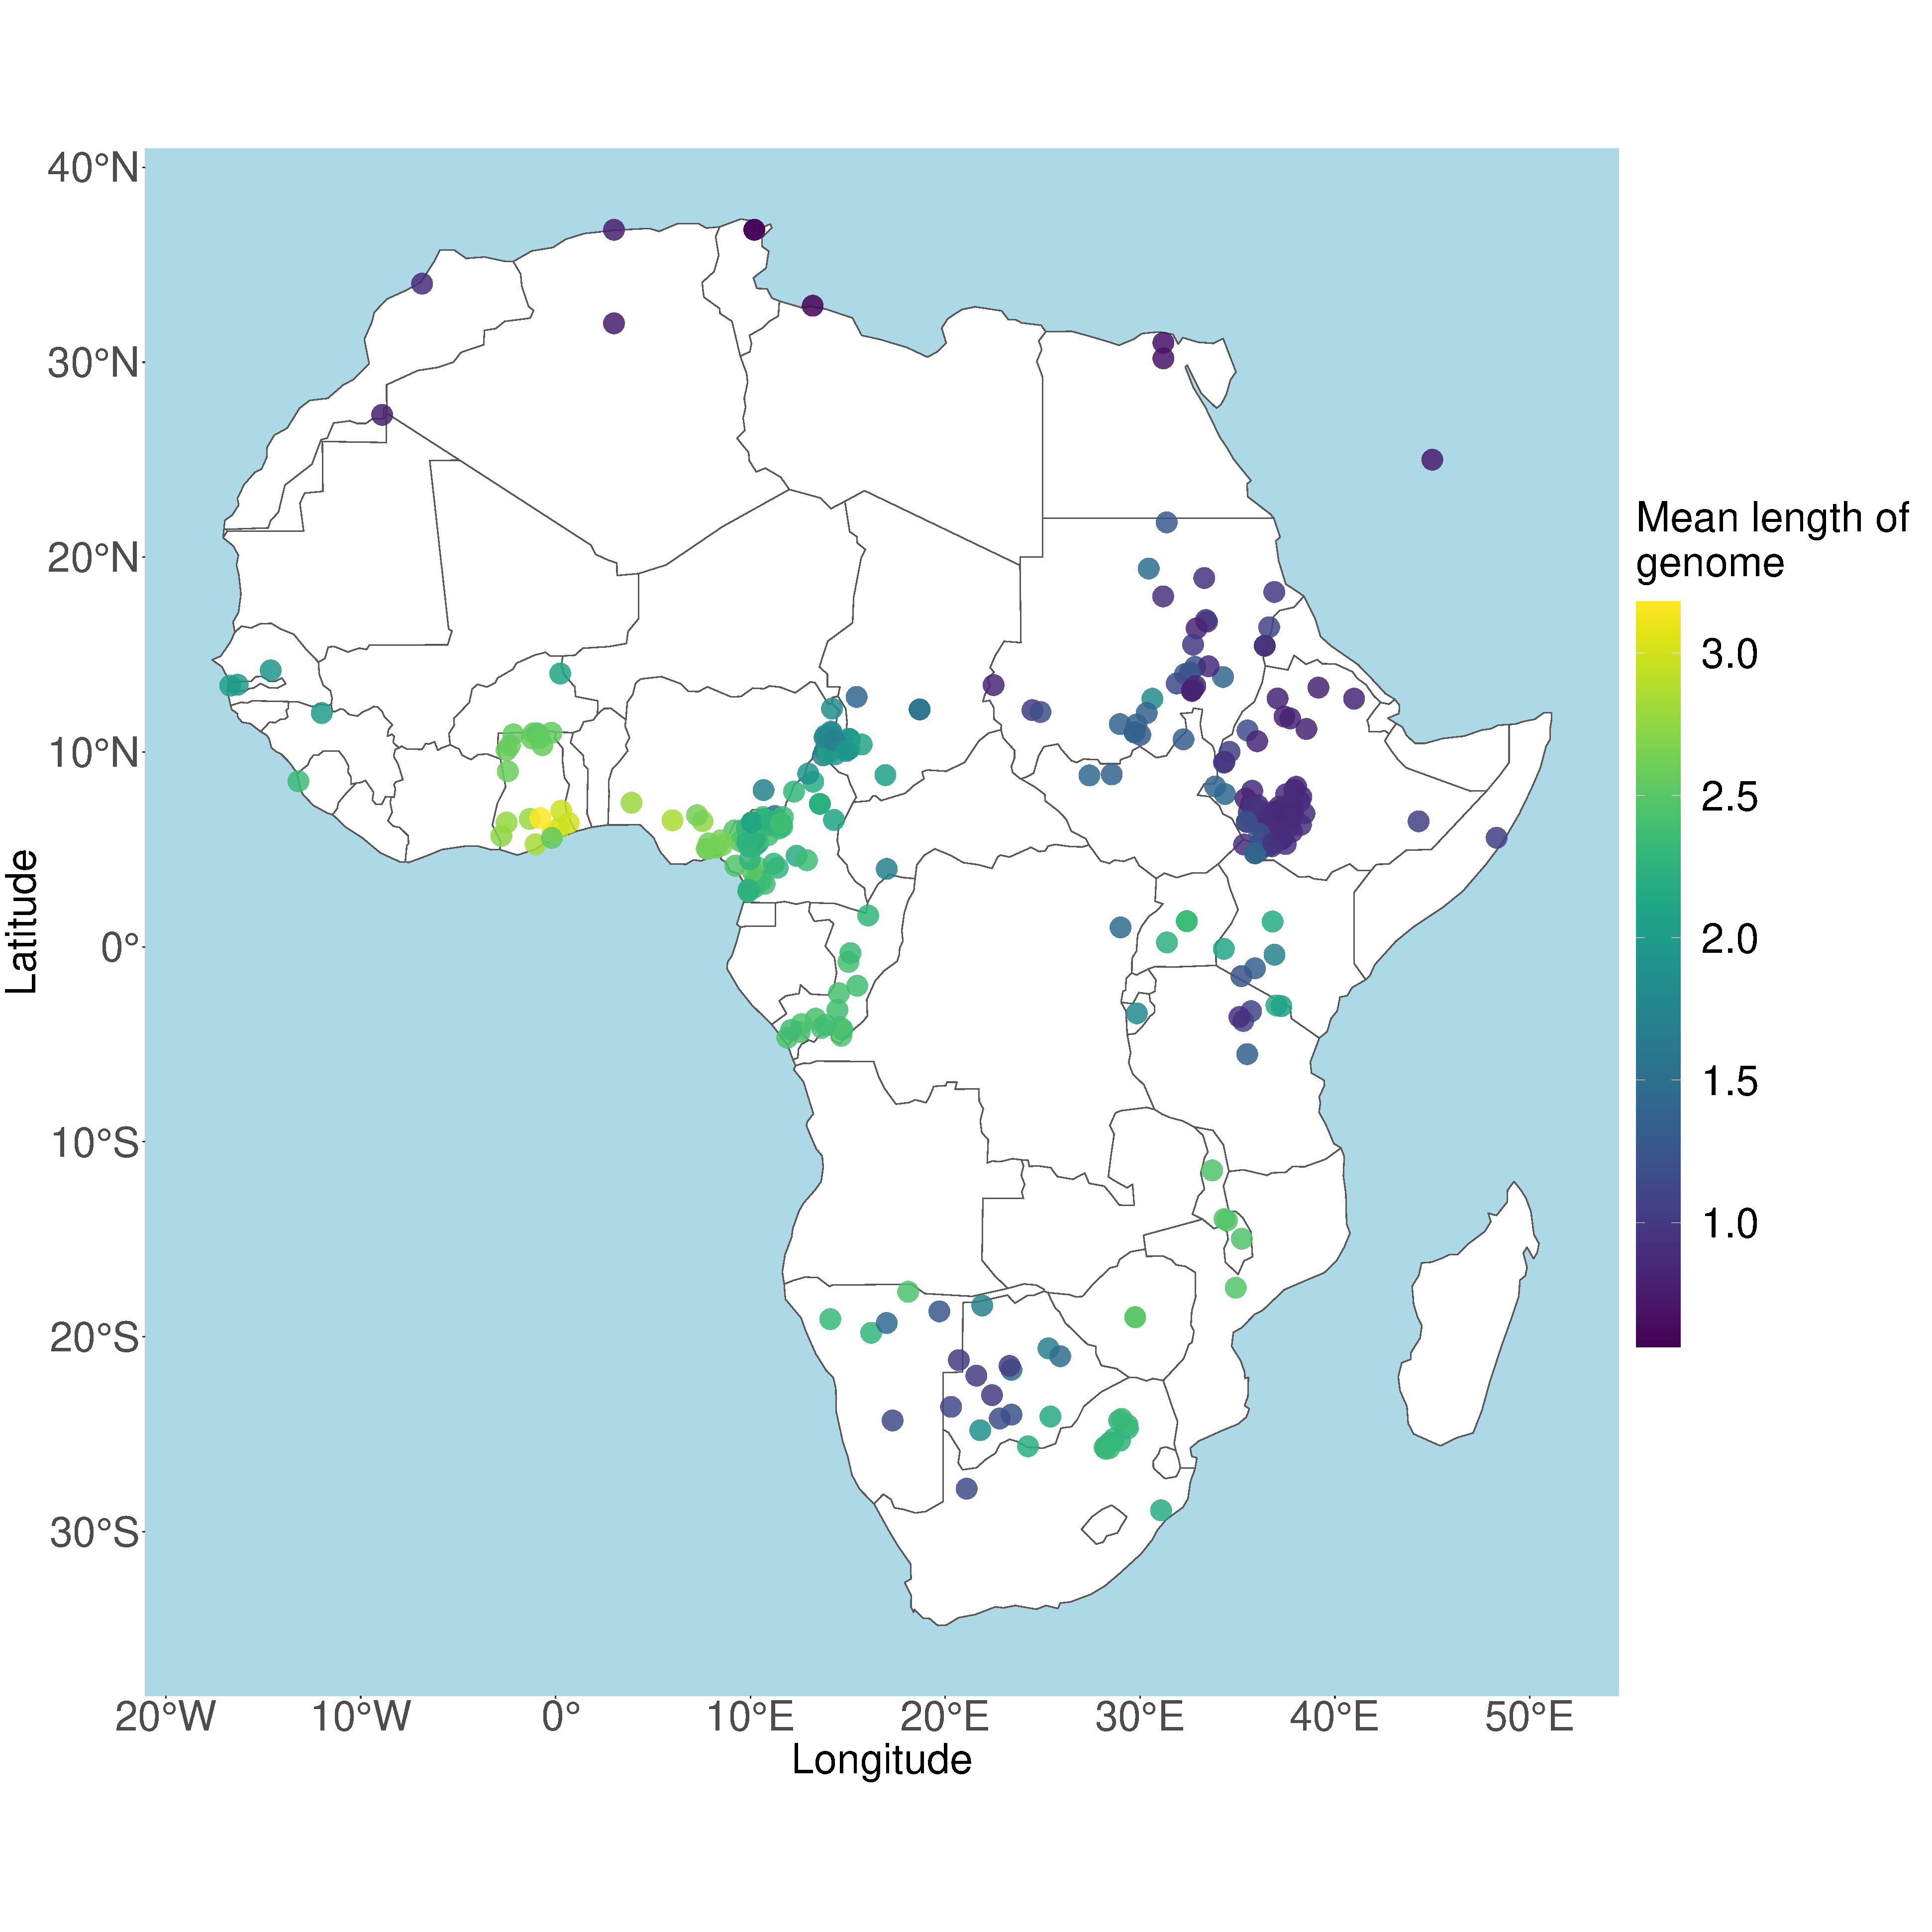
\includegraphics[width=1.0\textwidth]{../images/chapter3/haplotype_sharing_map.pdf}
    \caption{Map of haplotype donation to U.K. Biobank individuals. Each point represents a different African population. Colour corresponds to the mean length (cM) that populatation donated to all African U.K. Biobank individuals.}
    \label{fig:haplotype_sharing_map_zoomed_II}
\end{figure}

The map supports the findings from the PCA in Fig. \ref{fig:PCA_chunklengths_HumanOrigins_U.K.Biobank}; the populations with the largest contribution are those from West Africa (Fig. \ref{fig:haplotype_sharing_map_zoomed_II}). In particular, populations from Ghana and Nigeria contribute the most to the ancestry of Biobank individuals. On the other hand, populations in east and north Africa contribute relatively little, with southern / south-east Africa being approximately intermediate. This is consistent with two different historical events. 

Firstly, it is known from historical and genetic studies that a majority of the individuals who were forcibly transported from Africa to the Americas during the transatlantic slave trade were from the west coast of Africa \cite{micheletti2020genetic}. Given the U.K. Biobank sample contains many individuals who were either born in, or trace their ancestry from the Caribbean, a region that had a large influx of slaves \cite{rawley2005transatlantic}, we would expect there to be a large contribution of ancestry from west Africa. Secondly and more recently, there has been a relatively large amount of historical immigration from countries in west Africa, such as Ghana and Nigeria, to the U.K \cite{banton1953recent}. Although there are a number of immigrants from other parts of Africa, reflected in the non-zero contributions from other ethnic groups, these contributions are small compared to those from West Africa.

I performed the same visualisation using the painting using imputed SNPs and the ancestry distribution was qualitatively the same. 

I used SOURCEFIND to infer the proportion of ancestry that each UK Biobank individual shares most recently with each of the 535 surrogate groups, as this accounts for uneven donor population sizes. A map of proportions is given in Fig. \ref{fig:SF_props_map}, with each point corresponding to the mean percentage of ancestry of that particular group across all African U.K. Biobank individuals. Similar to the copyvector map, the ancestry is focused around Nigeria and Ghana, with Yoruba (39.8\%) and Ghana Fante (7.31\%) having the highest mean proportions. The distribution of colour on this figure is focused around a smaller number of populations compared to Fig. \ref{fig:haplotype_sharing_map_zoomed_II}. This is because SOURCEFIND attempts to narrow down the set of populations which most likely contribute towards the ancestry of a given individual and so appear `cleaner' than raw ChromoPainter results. 

\begin{figure}[htp]
    \centering
    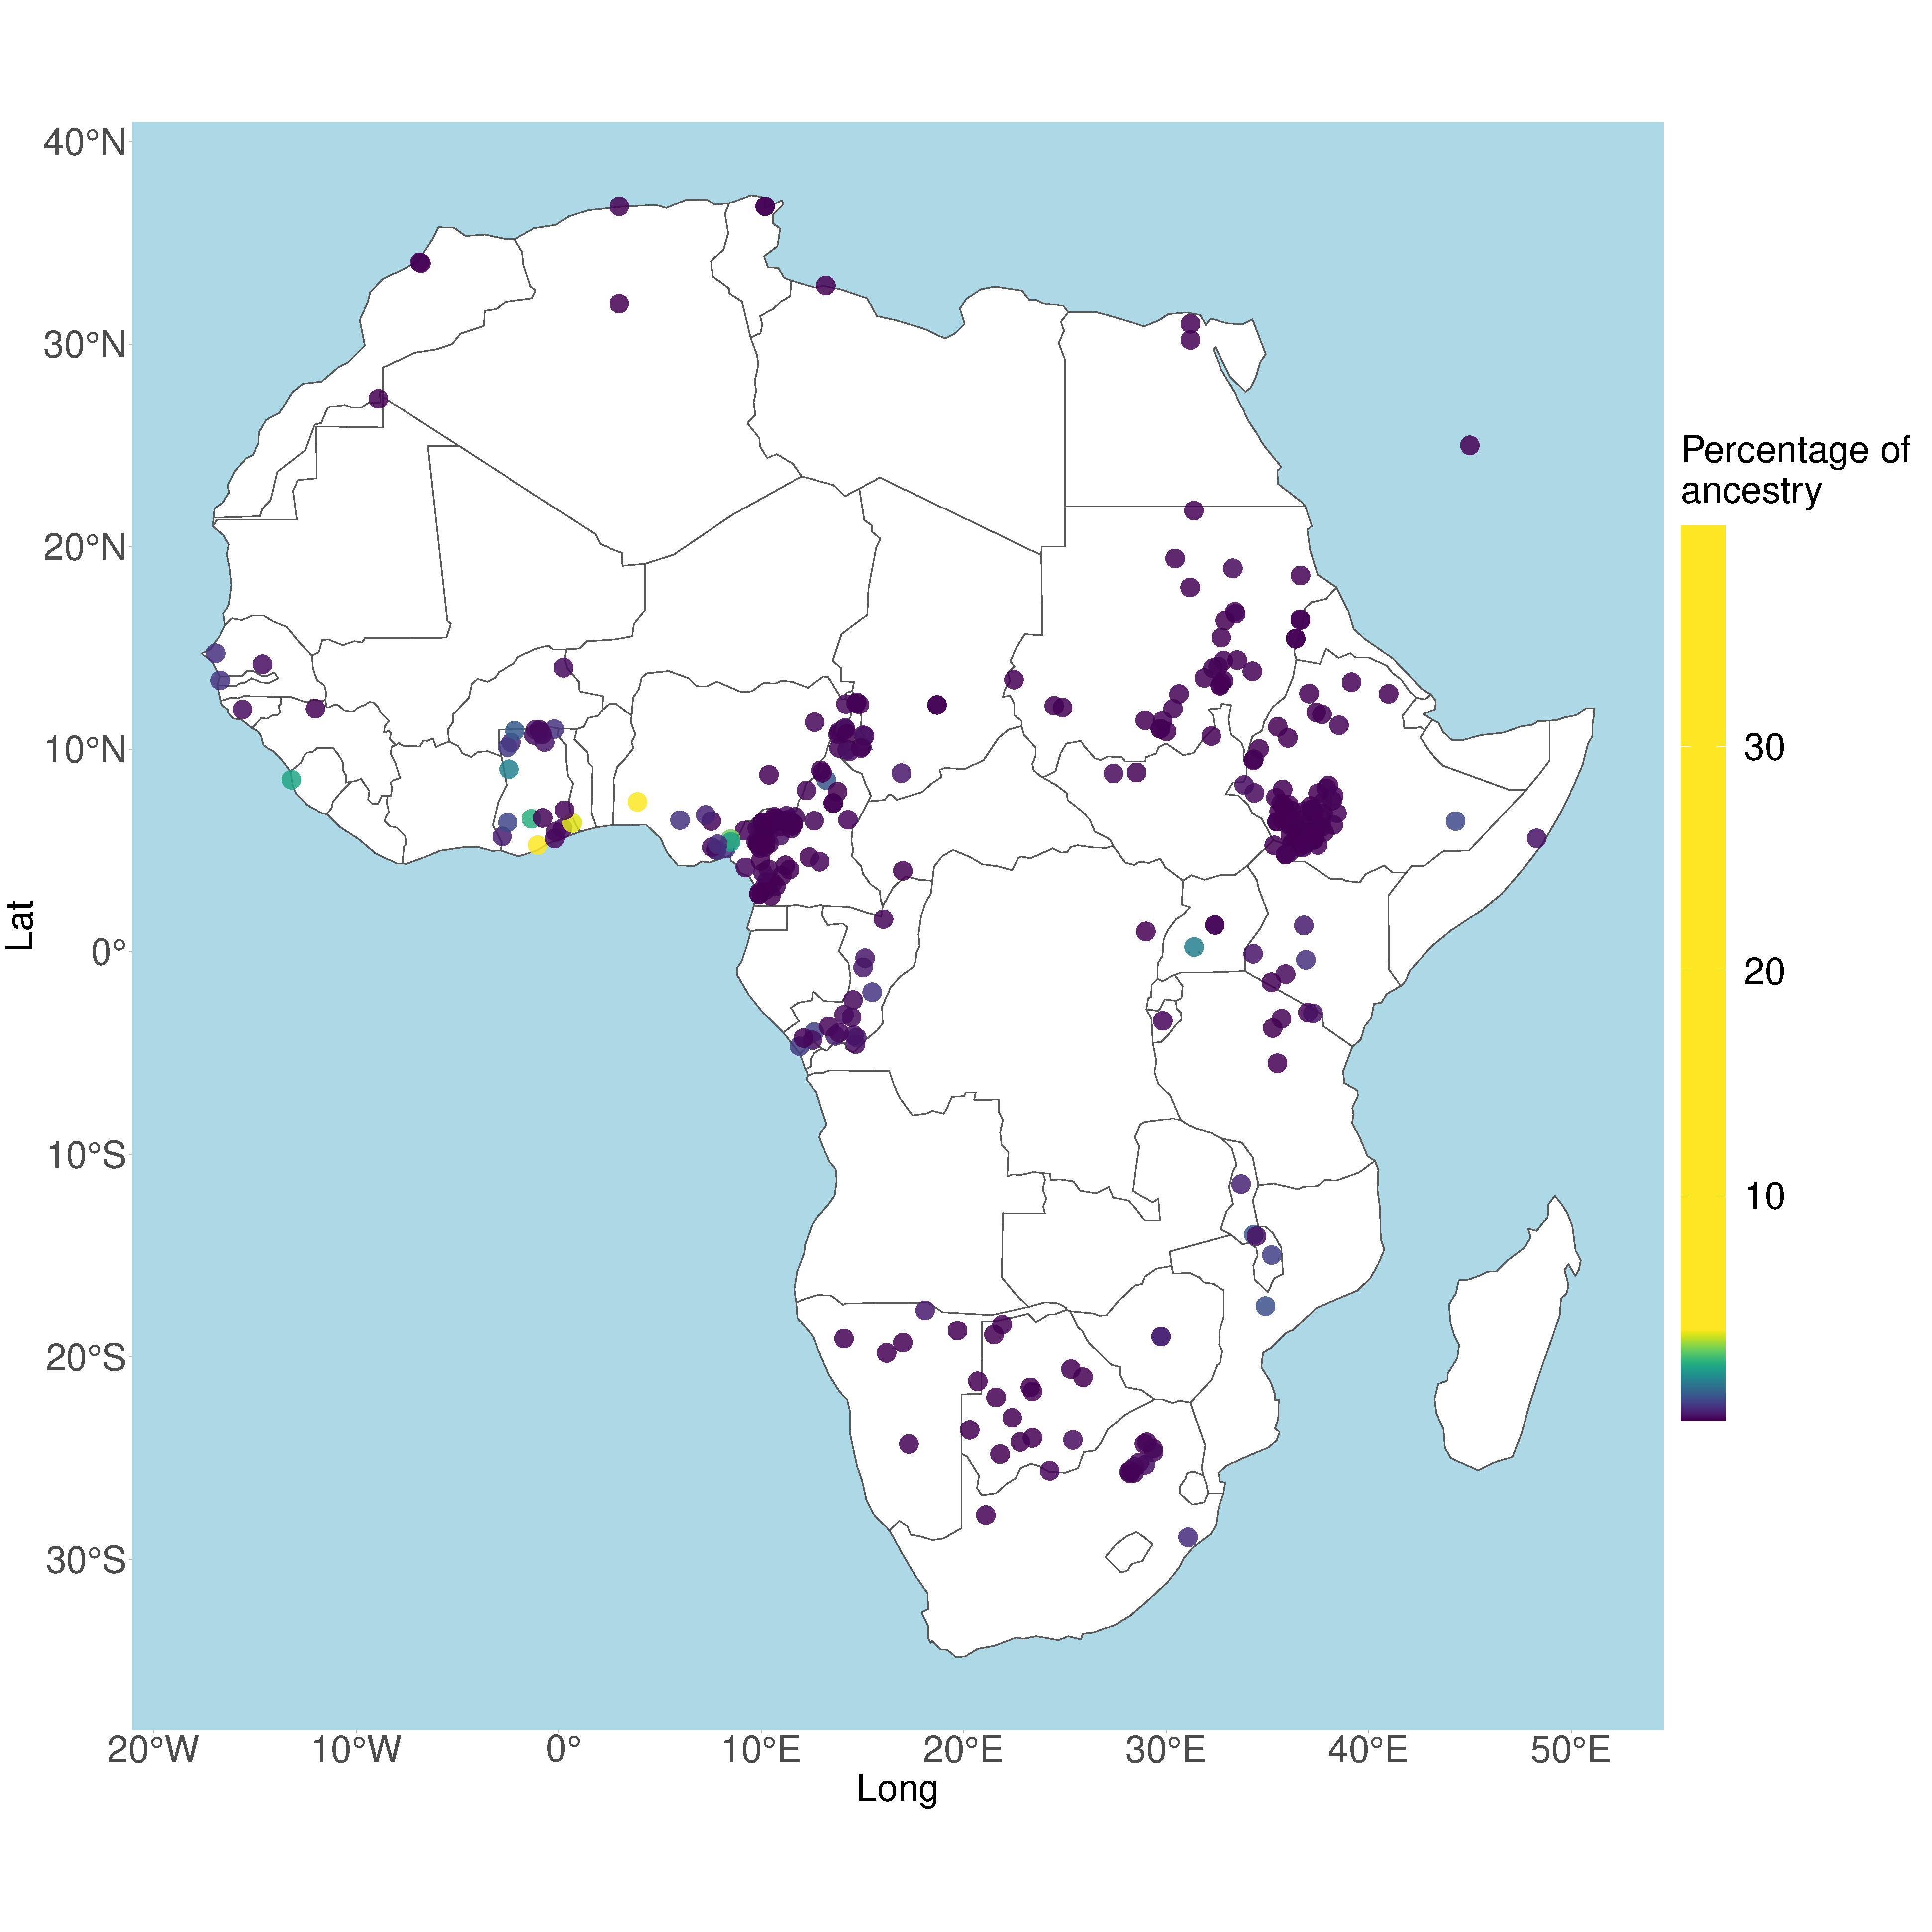
\includegraphics[width=1.0\textwidth]{../images/chapter3/SF_props_map.pdf}
    \caption{Map displaying the mean proportion of SOURCEFIND estimated ancestry of each African reference population within U.K. Biobank individuals. Each point is an African reference population with the colour corresponding to the mean ancestry proportion for that population across selected U.K. Biobank individuals. The colour-bar has been rescaled as two populations, Yoruba and Ghana\_Fante have substantially higher proportions than all other populations.} 
    \label{fig:SF_props_map}
\end{figure}


Fig. \ref{fig:SF_props_distribution_top30} displays the 30 ethnic groups with the highest mean proportions of ancestry within the U.K. Biobank individuals, and the distribution of values within each group. Yoruba was a clear standout for the most represented population;  3604/8309 individuals had at least 50\% Yoruba ancestry. This is compared to the next most common ancestry, Ghana\_Fante, which had an average of 7.3\% per person and 373/8309 individuals with at least 50\% ancestry. It is not clear what the reason for the large amount of Yoruban ancestry relative to all other populations is. One possible answer may come from considering the birth country of the U.K. participants. Of all the individuals for which we have country of birth data for (n=6190), more of them were born in the Caribbean (n=2263) relative to any other country. This should not be surprising given the history of migration from the Caribbean to the U.K. Of the individuals born in the Caribbean, over half were assigned to the Yoruban ethnicity, a much higher proportion than any other country of birth. Therefore, one could tentatively explain the abundance of Yoruba ancestry as resulting from the transatlantic Slave Trade, where individuals from the Yoruba ethnic group were taken to the Caribbean at a higher frequency than other nearby ethnic groups in the Human Origins reference. This may be in part because Yoruba is the second largest ethnic group in Nigeria and individuals belonging to it live primarily in coastal areas where the Slave Trade operated. The relatively large number of individuals from the Caribbean in the U.K. could thus have brought Yoruban ancestry to the U.K. 

\begin{figure}[htp]
    \centering
    \includegraphics[width=1.0\textwidth]{../images/chapter3/SF_props_distribution_top30.pdf}
    \caption{The 30 Human Origins populations which have the highest contribution to all U.K. Biobank individuals with at least 50\% African Ancestry, based on SOURCEFIND analysis. Each row of points contains 8476 individuals and their position corresponds to the percentage of ancestry from that population. }
    \label{fig:SF_props_distribution_top30}
\end{figure}

There are other instances of an over and under-representation of one ethnic group from a particular country (Fig. \ref{fig:all_countries_SF_props_pie_chart}). For example, Nigeria is dominated by a single ethnic group, despite having data for 31 different ethnic groups.  On the other hand, the individuals from Sudan are more evenly distributed across ethnicities. This may be caused because there are more reference ethnic groups in Sudan to assign individuals to. Further, it is known (personal communication N.Bird, 2021) that using the Human Origins dataset, there is inability to distinguish  between individuals in closely related Sudanese populations. 

\begin{figure}[htp]
    \centering
    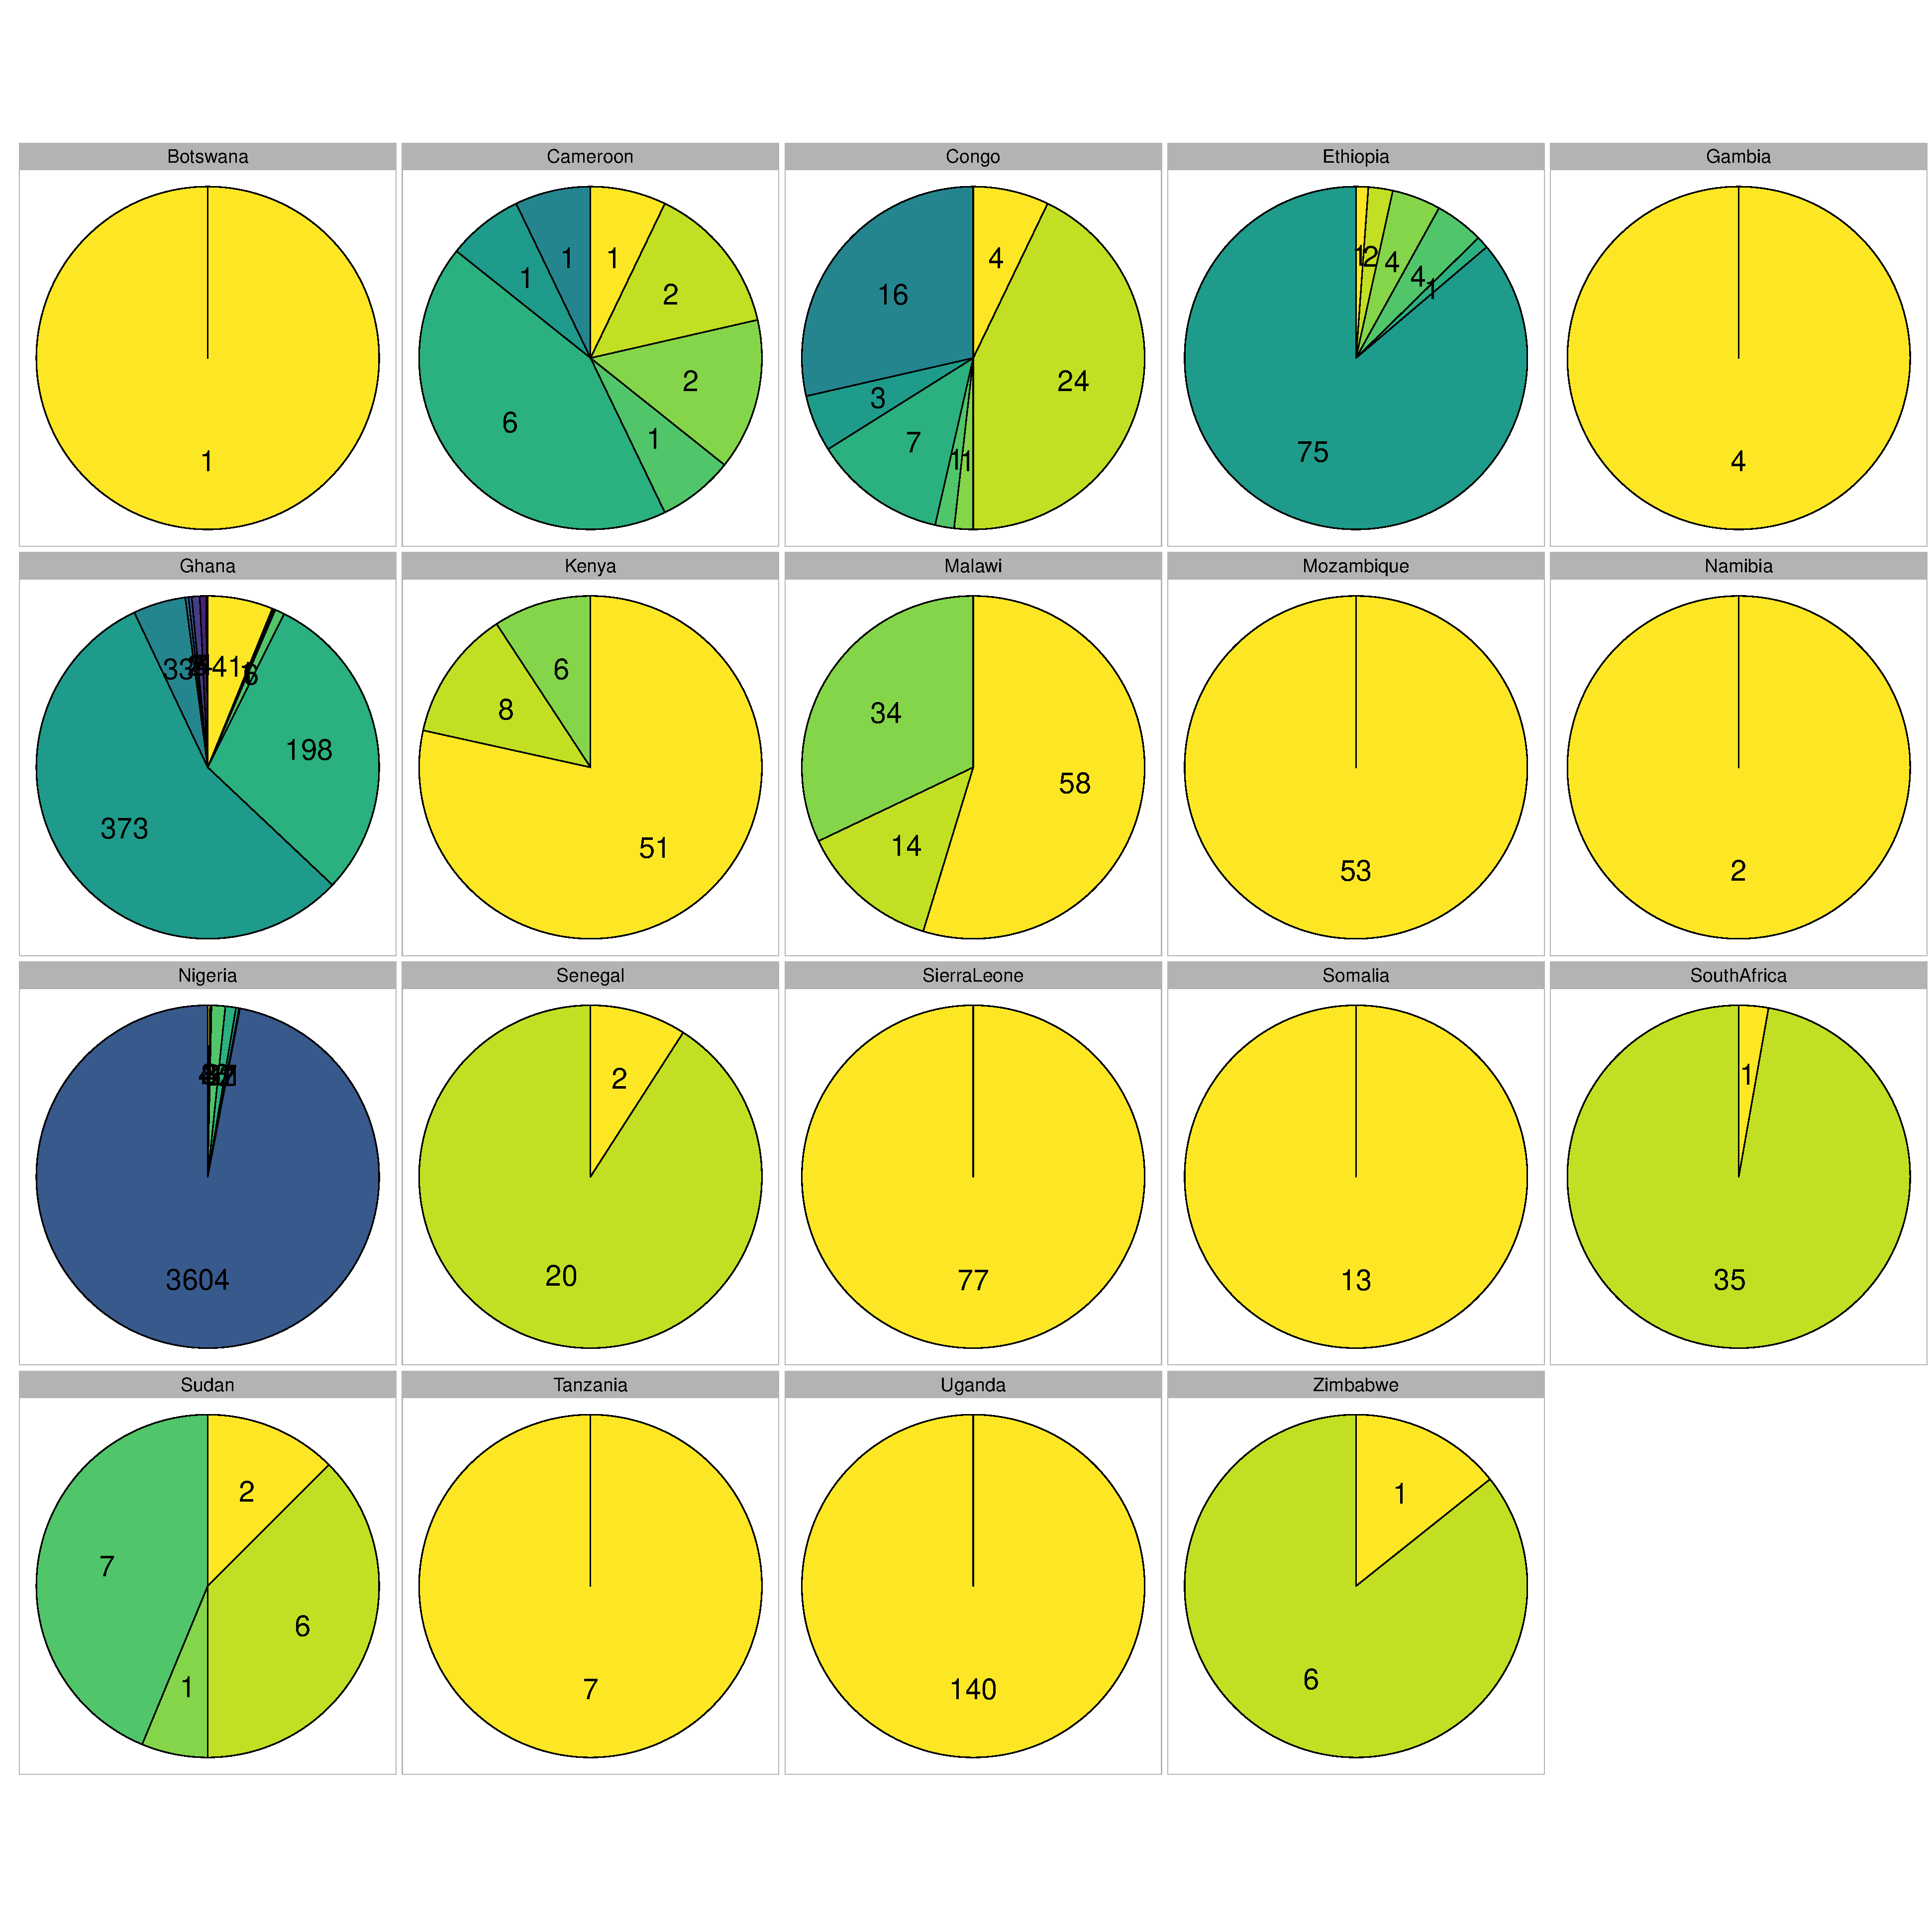
\includegraphics[width=1.0\textwidth]{../images/chapter3/all_countries_SF_props_pie_chart.pdf}
    \caption{Variation of individuals assigned to different ethnic groups by country of assigned group. Each panel represents all individuals assigned to an ethnic group from that country, with proportions of each pie corresponding to proportion of individuals of that ethnic group in that country. Numbers within each slice correspond to total number of individuals within a given ethnic group.}
    \label{fig:all_countries_SF_props_pie_chart}
\end{figure}

Some other patterns can be noted. Whilst many individuals have intermediate levels of ancestry from West African populations (e.g. Ghana\_Fante or Yoruba\_Yoruba), much fewer individuals have intermediate levels of Ethiopia\_Somali ancestry (Fig. \ref{fig:SF_props_distribution_top30}). This may be because Somalis are more recent immigrants to the UK and therefore tend to be less admixed with Europeans relative to other immigrant populations which have been in the U.K. longer and hence can be modelled as a mixture of almost entirely Ethiopia\_Somali ancestry. 

To test whether this was the case, I selected individuals assigned to either Ethiopia\_Somali, Yoruba or Ghana\_Fante and estimated their proportions of total African, European and Asian ancestry using SOURCEFIND. Individuals from Yoruba and Ghana\_Fante had, on average, 6.2\% and 5.2\% European ancestry respectively, whereas individuals from Ethiopia\_Somali had 0.21\% on average, suggesting they are indeed less mixed than other populations, which is consistent with them being more recent migrants. 

\subsection{Verifying painting accuracy} 
 
Not all individuals within the U.K. Biobank were born in the U.K.; visualising the ancestry distribution of these individuals allows ensures us that the painting is accurate and may reveal insights into population history. For instance, the ancestry distribution of individuals born in the Caribbean may provide evidence for where in Africa slaves forcibly transported to the Caribbean during the transatlantic slave trade originated from. This is important, as disembarkation records from the Slave Trade are often sparse, meaning many people with African ancestry who currently live in the Americas may not have knowledge of where their ancestors originated from.

I subsetted the coancestry matrix to contain only U.K. Biobank individuals who provided data on birth location (n=6153/8472). We would expect that individuals who were born in a particular country would copy the most from reference populations from that country. For example, we would expect individuals who were born in South Africa to copy the most from sampled Bantu and Zulu ethnic groups from South Africa. This may not always be the case, as some ethnic groups have crossed borders in their history,  or we may not have sampled representative groups from some countries, but it may broadly be expected to be true. We also have birth place data for individuals who were not born in Africa (e.g. the Caribbean and Brazil). 

\begin{figure}[htp]
    \centering
    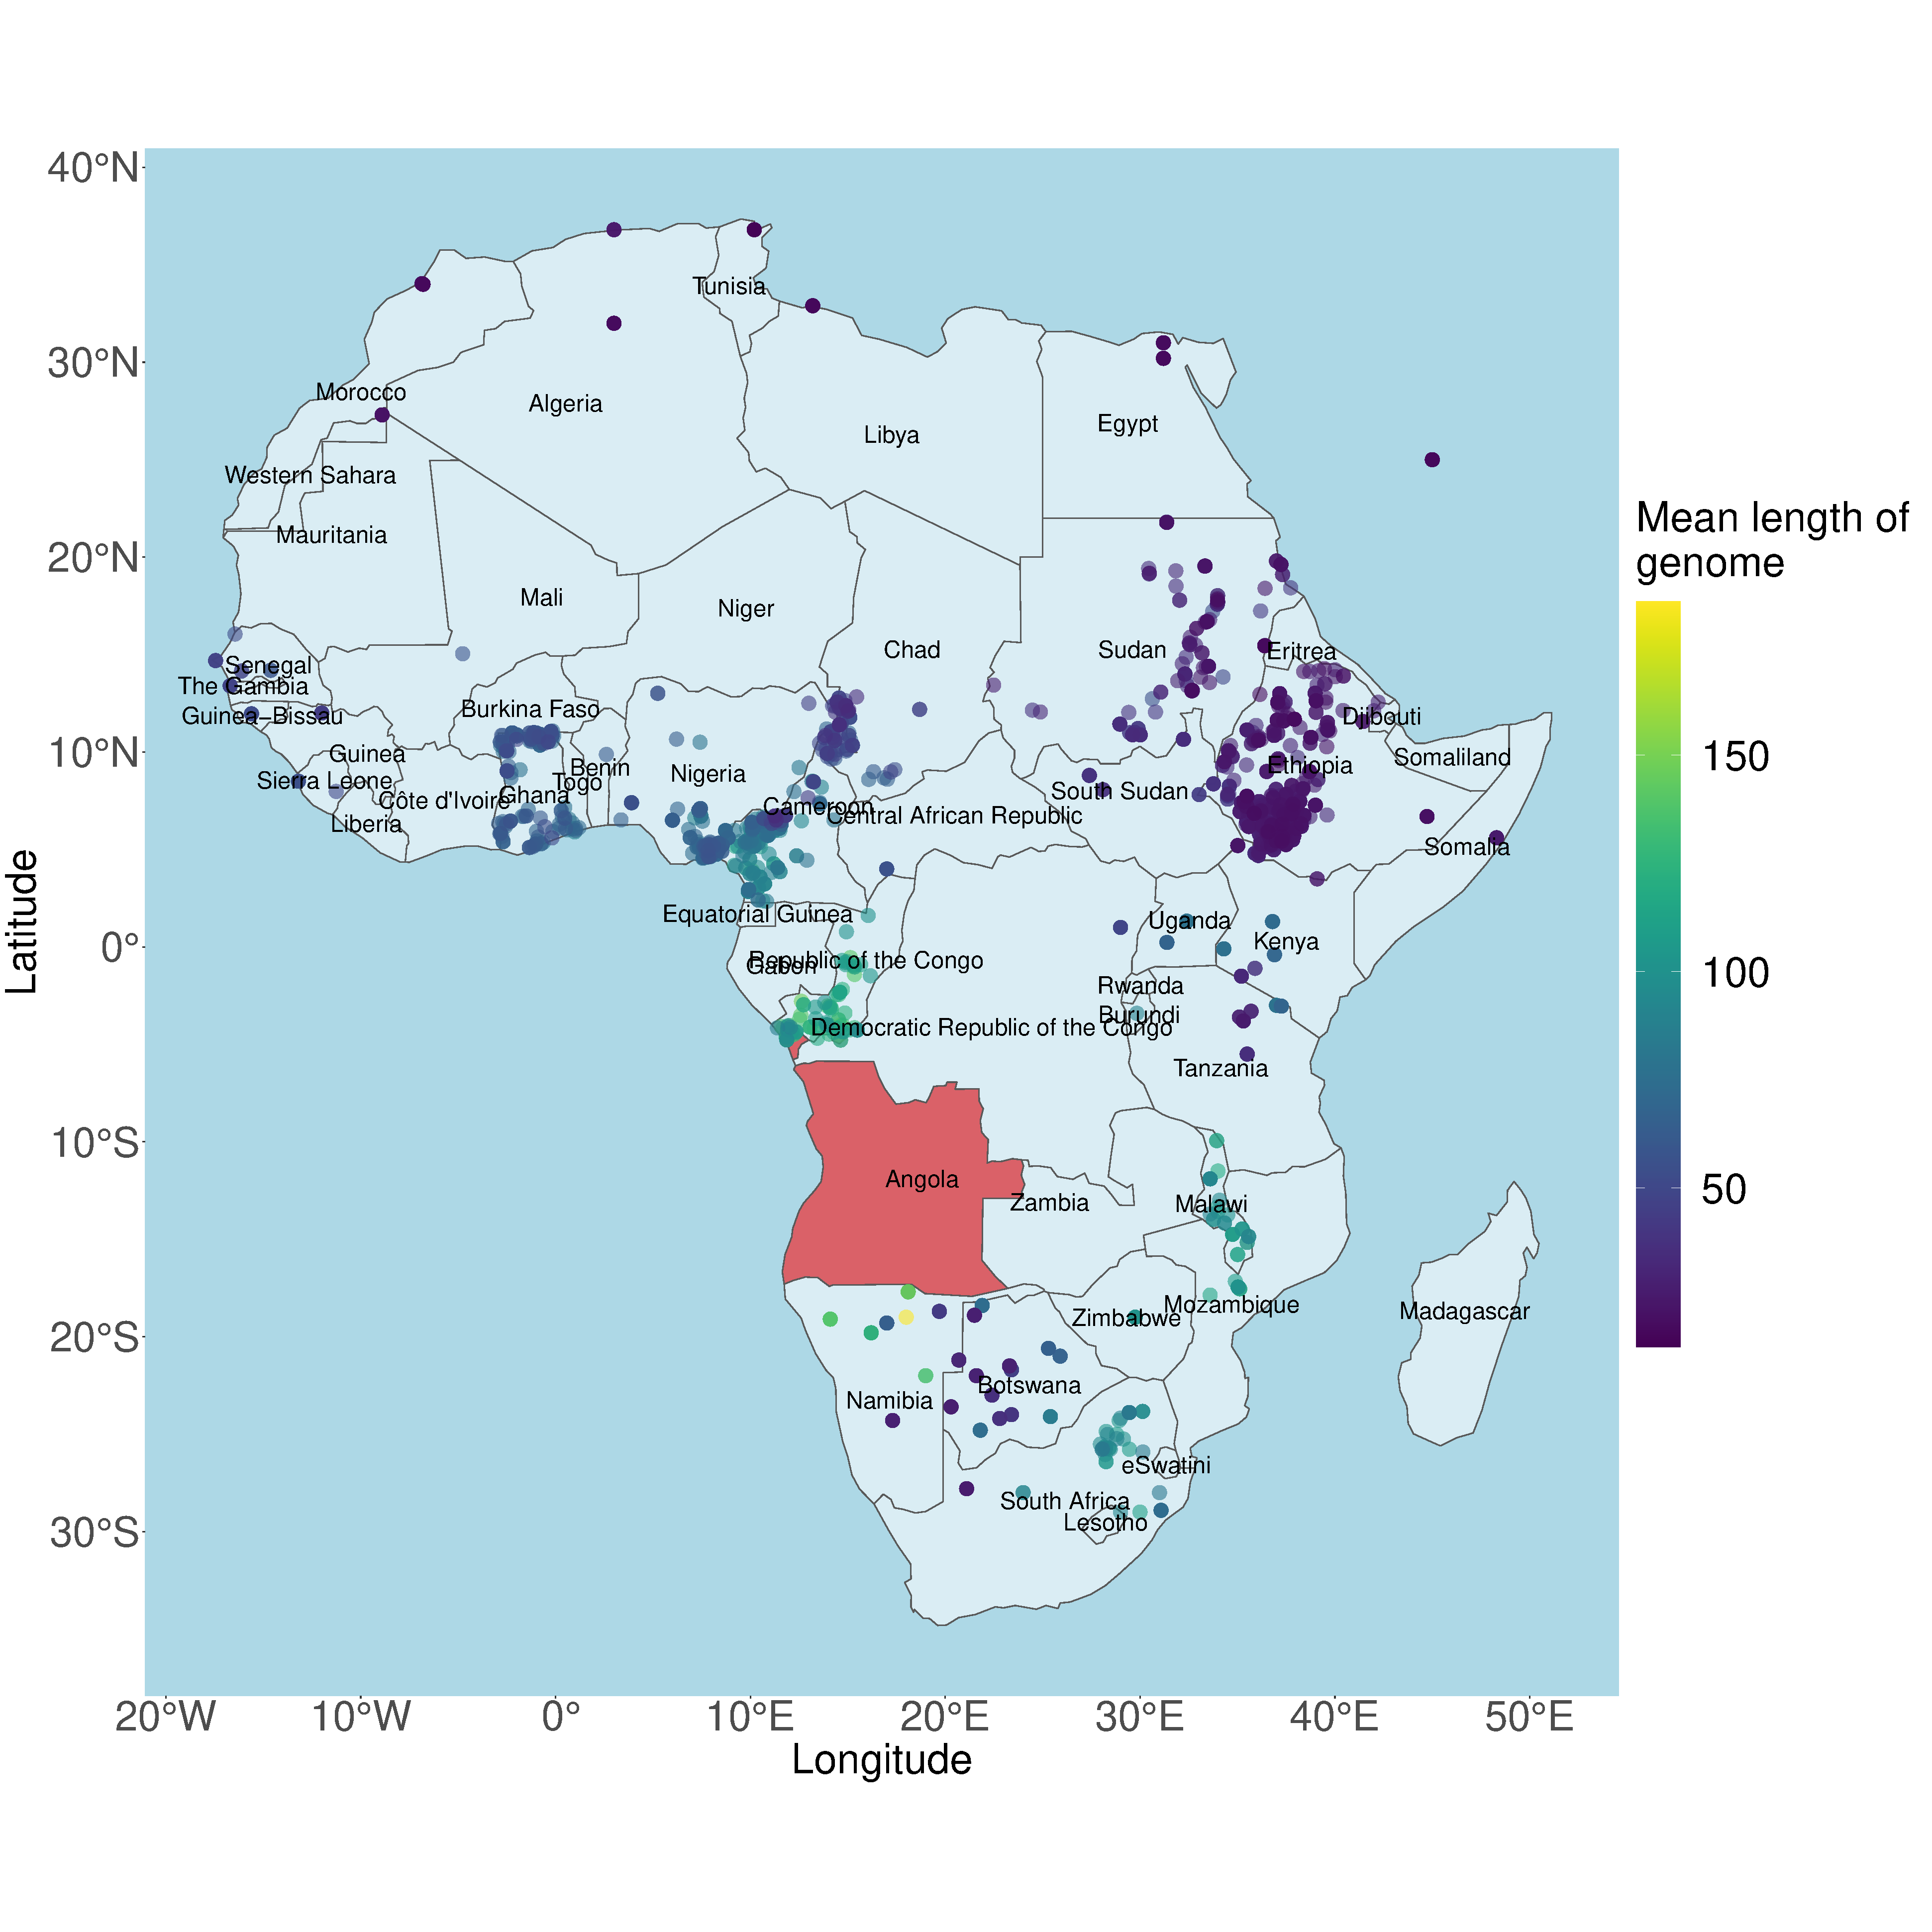
\includegraphics[width=1.0\textwidth]{../images/chapter3/haplotype_map_SouthAfrica.pdf}
    \caption{Map of haplotype donation to U.K. Biobank individuals born in South Africa. Each point represents one Human Origins population, coloured according to the summed amount of chunklengths that population donates to all U.K. Biobank individuals born in South Africa. }
    \label{fig:haplotype_map_SouthAfrica}
\end{figure}

Fig. \ref{fig:haplotype_map_SouthAfrica} shows the map of haplotype donation from reference groups to U.K. Biobank individuals born in South Africa. It is clear that reference populations from South Africa, in particular the Zulu ethnic group, contribute the most to these individuals. The pattern is qualitatively the same for all countries which had a reasonable number of donor populations, suggesting that the painting had good resolution down to at least the level of individual countries (Fig \ref{fig:country_of_origin_allInds}).

There are several interesting results. For example, there are 2,263 individuals who were born in the Caribbean; visualising the haplotype donation map for these individuals shows that they are primarily of West African ancestry (supplementary figure \ref{fig:haplotype_map_Caribbean}), consistent with historical evidence \cite{micheletti2020genetic}. Individuals born in Brazil have ancestry from further South, again consistent with historical evidence (supplementary figure \ref{fig:haplotype_map_Brazil}). Of the nine individuals born in Brazil, six of them had a majority SOURCEFIND component from an ethnic group in The Republic of the Congo. However, it should be noted that there is a relatively small sample size from individuals born in Brazil (n=9), and that these individuals may not be representative of the Brazilian population as a whole. 

As a formal test of the painting accuracy, I estimated SOURCEFIND ancestry proportions in each retained U.K. Biobank individual. An individual was `assigned' to a particular ethnic group if they had 75\% or more of their total ancestry from that group. If the country the assigned reference population is from matches the birth location of the individual, then I considered that a `success' and a `fail' otherwise. Individuals who were born in the U.K. or who had no birth country were excluded from this analysis. 75\% was chosen as an arbitrary threshold. 

\begin{figure}[htp]
    \centering
    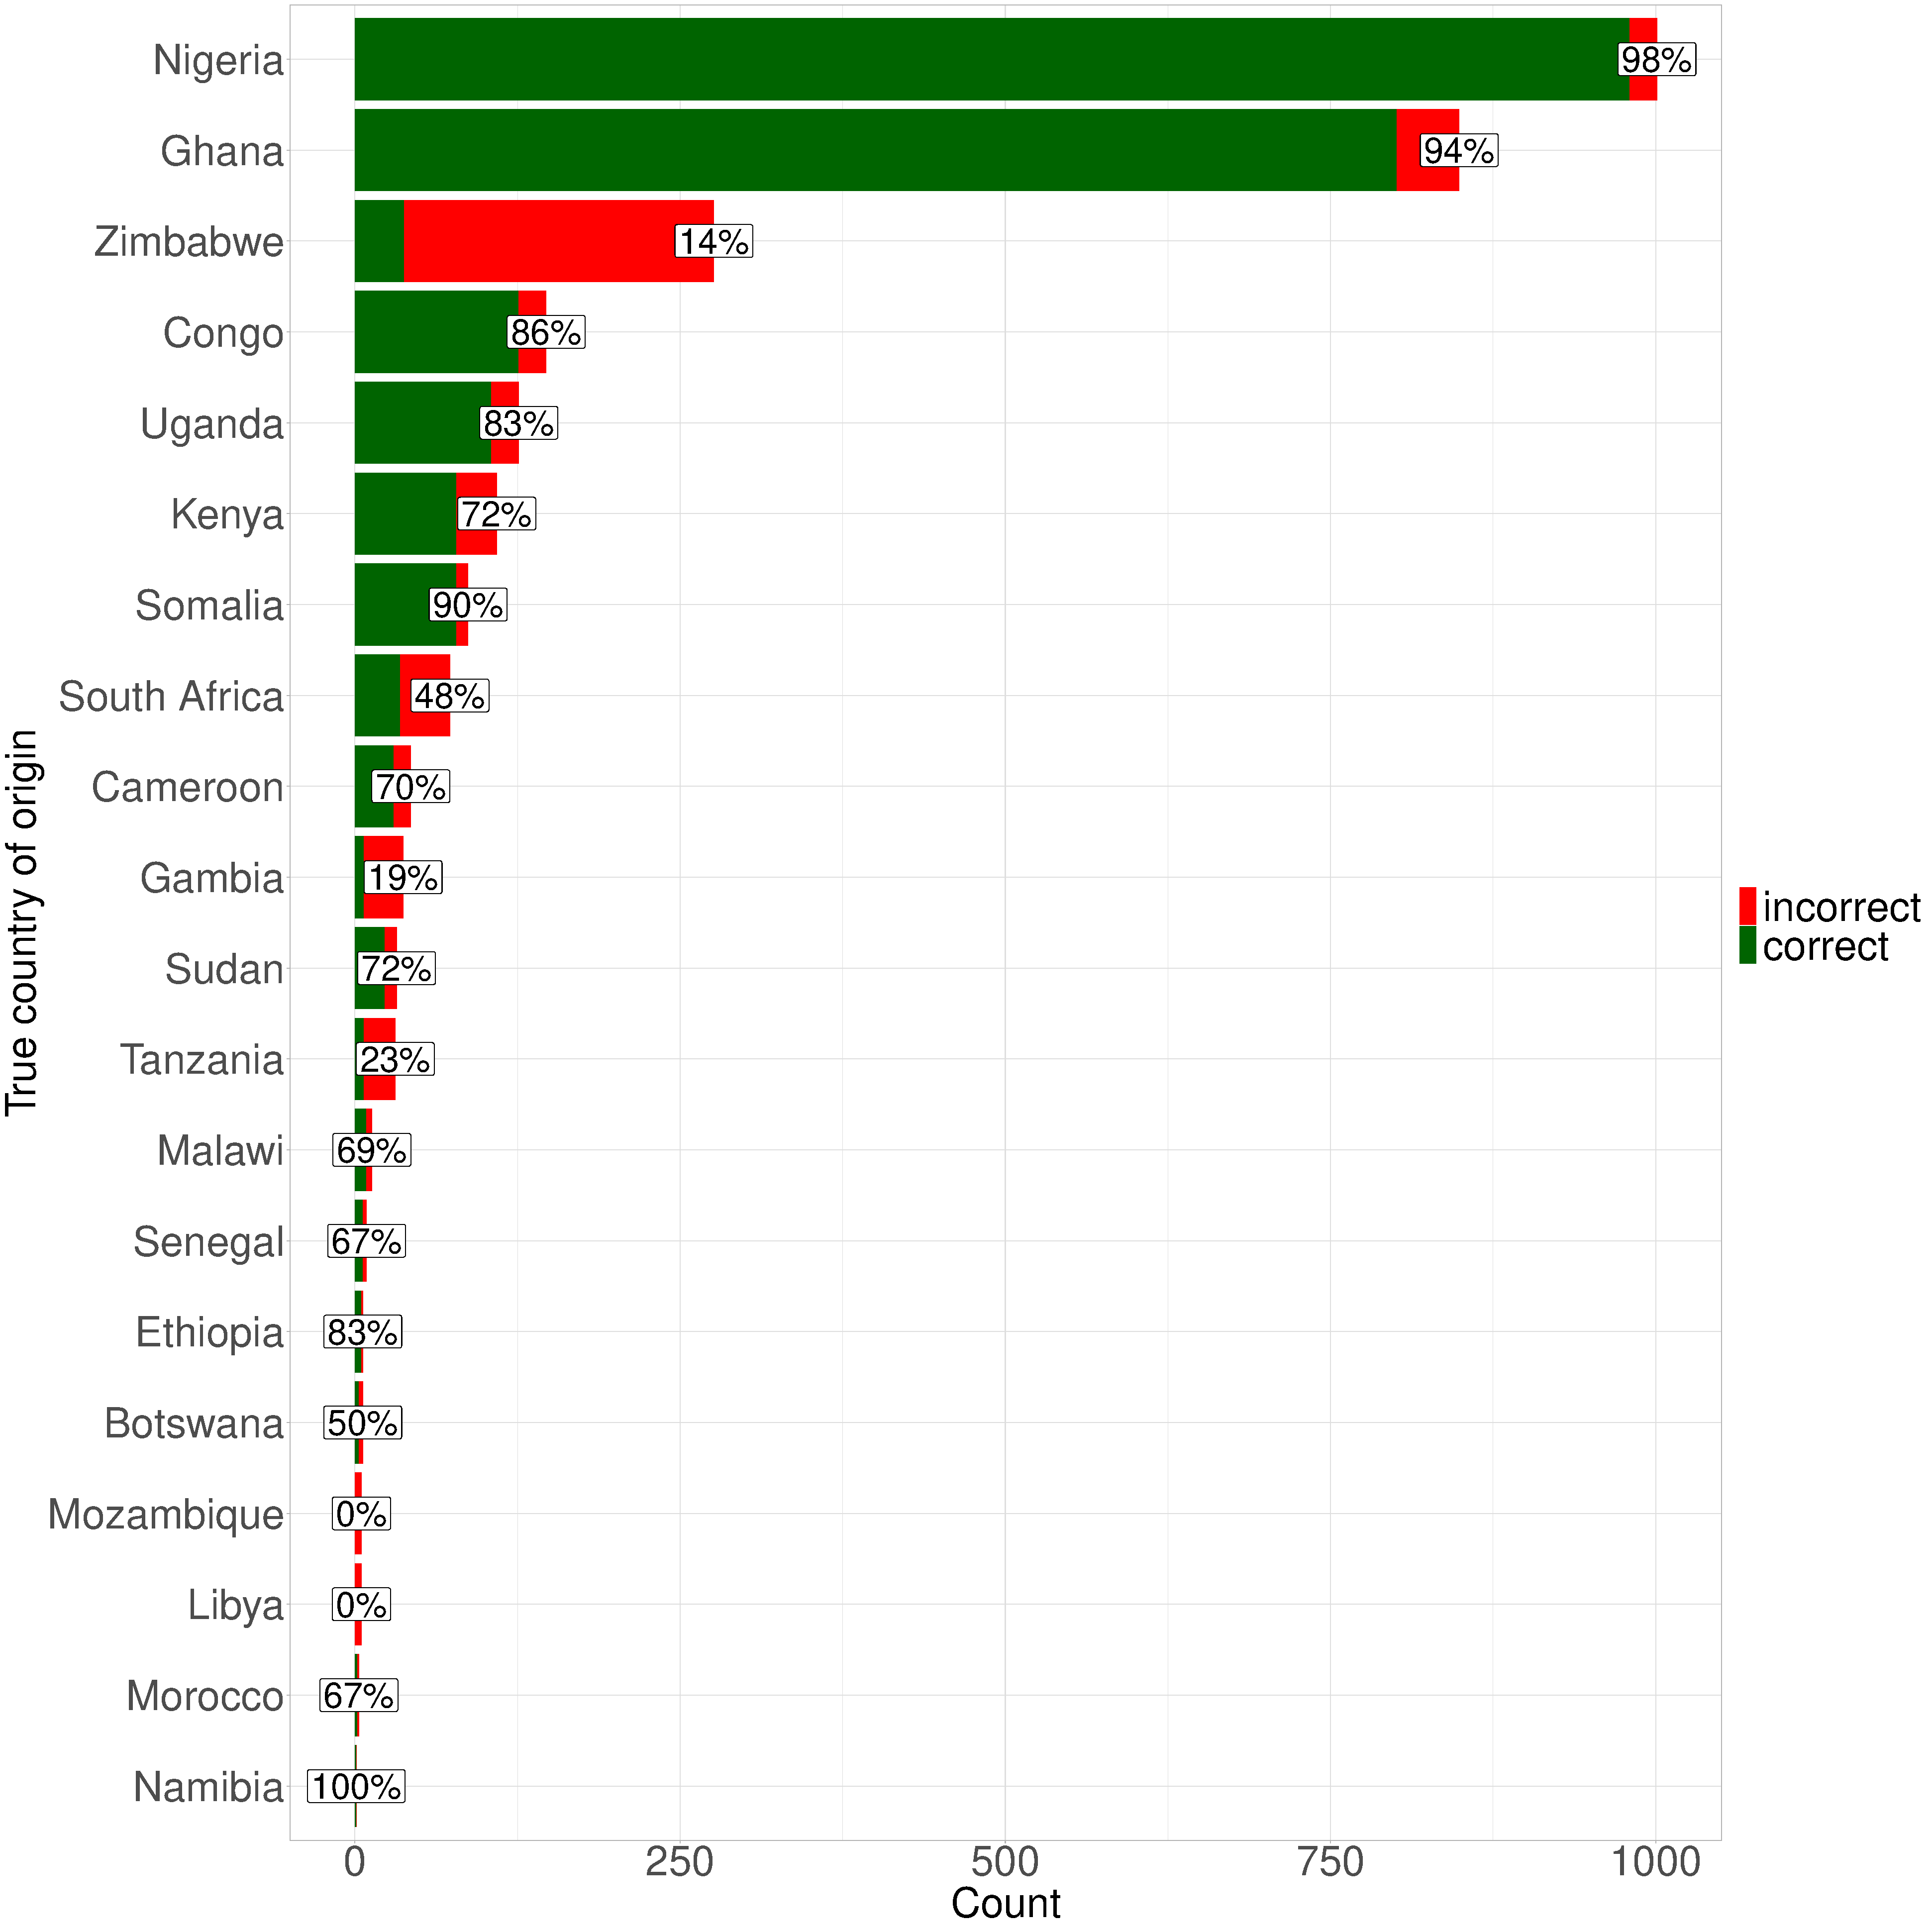
\includegraphics[width=1.0\textwidth]{../images/chapter3/country_of_origin_allInds.pdf}
    \caption{Correspondence of true birth country with estimated birth country. Each bar corresponds to a true birth country, with the length of the bar corresponding to the total number of people in our dataset born in that country. The green section corresponds to the total number of individuals where the birth country was correctly guessed and the red section to those who were incorrectly guessed. Percentage labels give percentage correct for that country.}
    \label{fig:country_of_origin_allInds}
\end{figure}

The overall accuracy at predicting birth location across all individuals was 81.63\%, suggesting there was substantial information within the coancestry matrix. For certain countries where there was large number of surrogate populations, such as Ghana and Nigeria, the prediction accuracy was high. For other countries, the prediction accuracy was much lower. For example, Tanzania, which is only represented by a single reference population, had a prediction accuracy of 23\%. Zimbabwe had by far the lowest prediction accuracy (14\%) out of countries with more than 100 U.K. Biobank individuals. Of the 266 individuals born in Zimbabwe, 194 were assigned to an ethnic group from outside Zimbabwe; 74 to Malawi\_Chewa, 71 to Mozambique\_Mozambique and 49 to Malawi\_Yao. Individuals from the ethnic groups from Malawi are found across Malawi, Zimbabwe and other countries, showing the possible weakness of this approach which aims to categorise individuals into a single country, as ethnic groups often transcend countries. Indeed we only have data from one (partially) Zimbabwean group, the Zulu, who may not well-reflect the ancestors of U.K. Biobank participants born in Zimbabwe.

I performed the same analysis but using the data which had been imputed. This stands as a practical test of whether it is preferable to impute or retain a smaller number of non-imputed SNPs when estimating country-level haplotype variation. This yielded an accuracy of 81.89\%, a value almost identical to that obtained with the dataset containing approximately 70,000 non-imputed SNPs, despite my earlier results indicating that sub-country population assignment results are less accurate if using imputed data due to reference bias (Table \ref{table:TVD_copying}). This may be because this broad-scale assignment of individuals to countries is not as affected by imputation as a more subtle dissection of sub-country ancestry. To test whether this is the case, I took all ethnic groups from Nigeria, Cameroon and Ghana in the Human Origins dataset which had five or more individuals (n=51 populations, n=1203 individuals), and for each individual, estimated ancestry proportions of each of the 51 populations. I performed this analysis for both datasets containing no imputed SNPs and 70\% imputed SNPs. For each dataset, I took the average proportion of ancestry for each ethnic group across all individuals. 

Fig \ref{fig:SOURCEFIND_imp_nonimp} shows that there are substantial differences between the proportions obtained from imputed and non-imputed datasets, showing sub-country assignment is affected by imputation. In particular, there is less variance across the proportions for the imputed dataset (var=0.67) relative to the non-imputed dataset (var=0.87). This is clear on the figure, as there are many population bunched around the 2\% point for the imputed dataset; the same populations are spread across a wider range of values for the non-imputed dataset. 

\begin{figure}[htp]
    \centering
    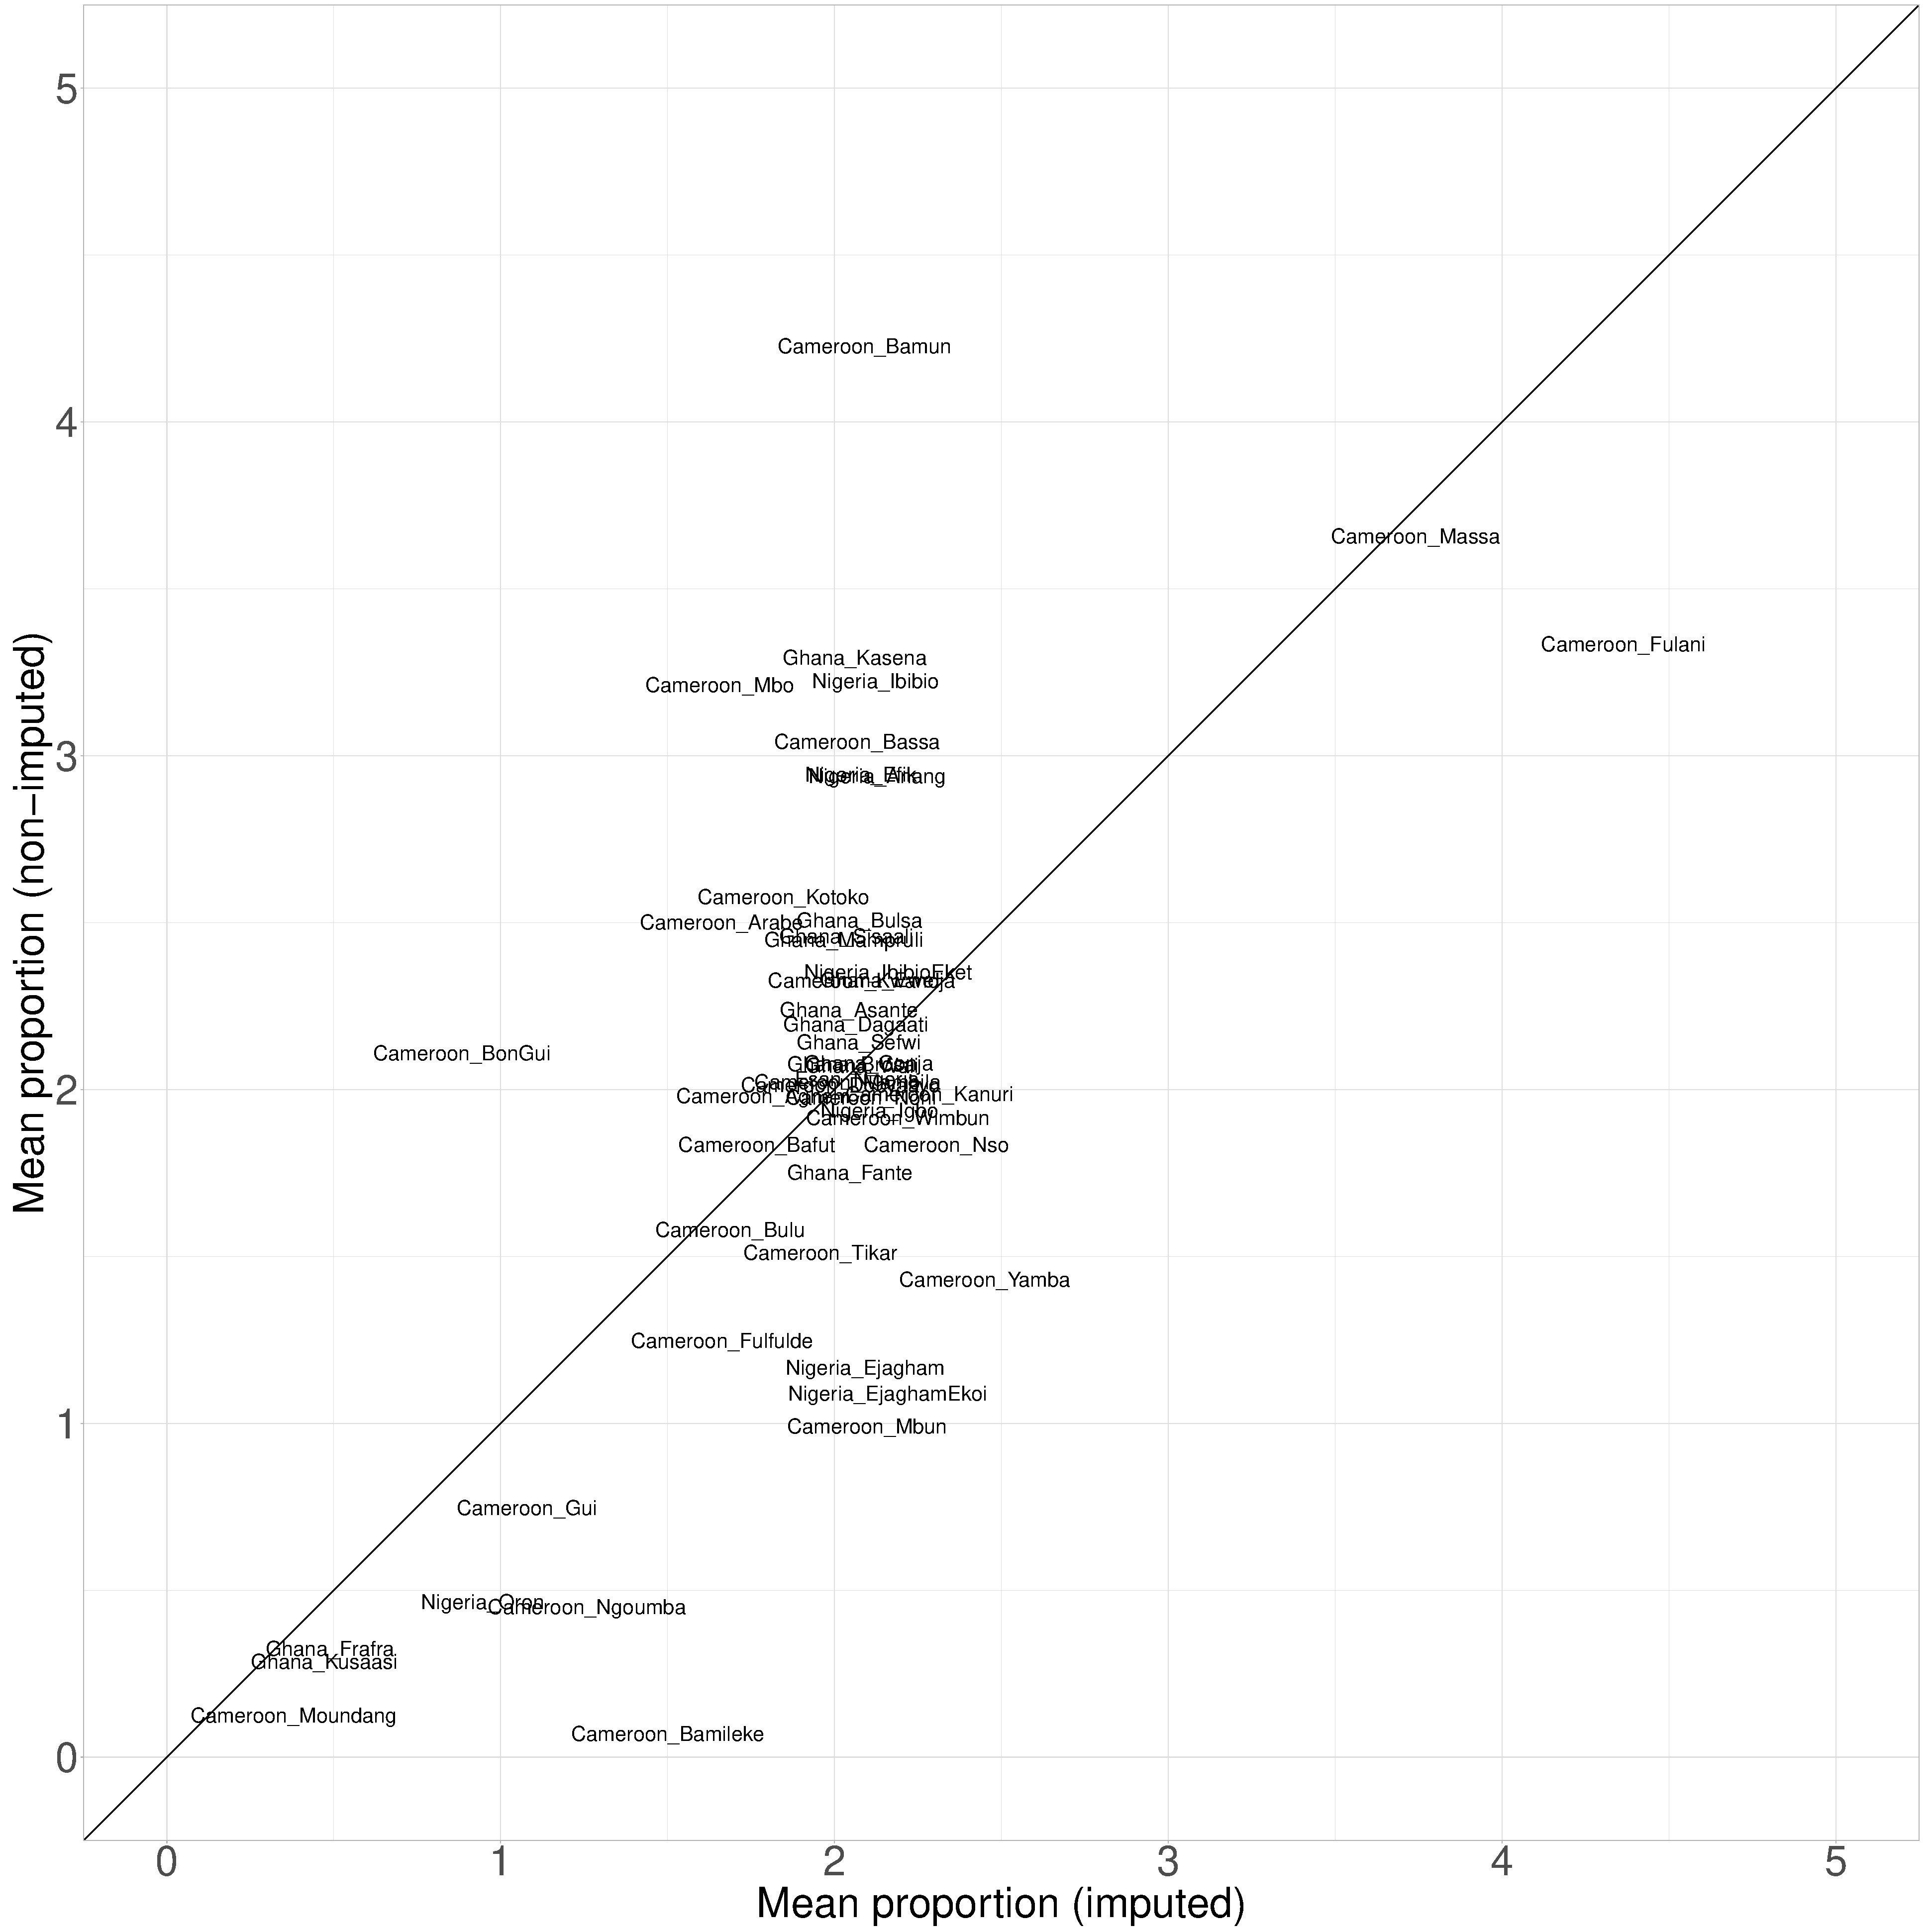
\includegraphics[width=1.0\textwidth]{../images/chapter3/SOURCEFIND_imp_nonimp.pdf}
    \caption{Mean ancestry proportions averaged across 1203 individuals from Ghana, Nigeria and Cameroon of 51 populations from the same countries. Proportions obtained from data containing 70\% imputed SNPs (x-axis) and no imputed SNPs (y-axis).}
    \label{fig:SOURCEFIND_imp_nonimp}
\end{figure}


\subsection{Patterns of African ancestry across the U.K.}

The U.K. Biobank dataset contains data on the testing centre that each individual registered at. I used this information to determine whether there was structure in how individuals with recent African ancestry are distributed across the U.K. There were no apparent outliers in terms of any centres with substantially larger proportion of individuals who had at least 50\% African ancestry than others (Supplementary Fig. \ref{fig:testing_centre_afr_prop}). However, as expected, centres in large cities such as Barts, Croydon and Hounslow (London), Birmingham and Manchester had the highest proportion of individuals with at least 50\% African ancestry.

I then plotted the distribution of people with recent ancestry related to African ethnic groups at different centres on a map of the U.K (Fig. \ref{fig:SF_props_pie_chart_entropy_map}). No clear pattern was apparent, other than Yoruban ancestry dominating most centres, with some smaller testing centres only containing individuals inferred as having Yoruba-related ancestry.  
 
I estimated the information entropy, $E$, of each assessment centre based on the SOURCEFIND proportions, similar to previous work performed by van Dorp et al (2018), who used the principle of entropy to determine the extent to which individuals from different ethnic groups were scattered across different clusters \cite{van2019genetic}.

To evaluate the extent to which individuals assigned to each ethnic group registered at different testing centers, I calculated entropy given by Schutze et al (2008) as $\sum_{i=1}^{L} [p_{i,j} \cdot log(p_{i,j})]$ \cite{schutze2008introduction}, where $p_{i,j} = \frac{m_{i,j}}{m_{j}}$, $m_{ij}$ is the number of individuals from testing center $j$ assigned to ethnic group $i$ and $m_{j}$ is the number of ethnic groups to which individuals from center $j$ are assigned. Testing centres in large cities such as London and Birmingham had the highest information entropy, consistent with prior expectations that large cities would contain a higher diversity of ancestries (Fig. \ref{fig:SF_props_pie_chart_entropy_map}). 


\begin{sidewaysfigure}
    \centering
    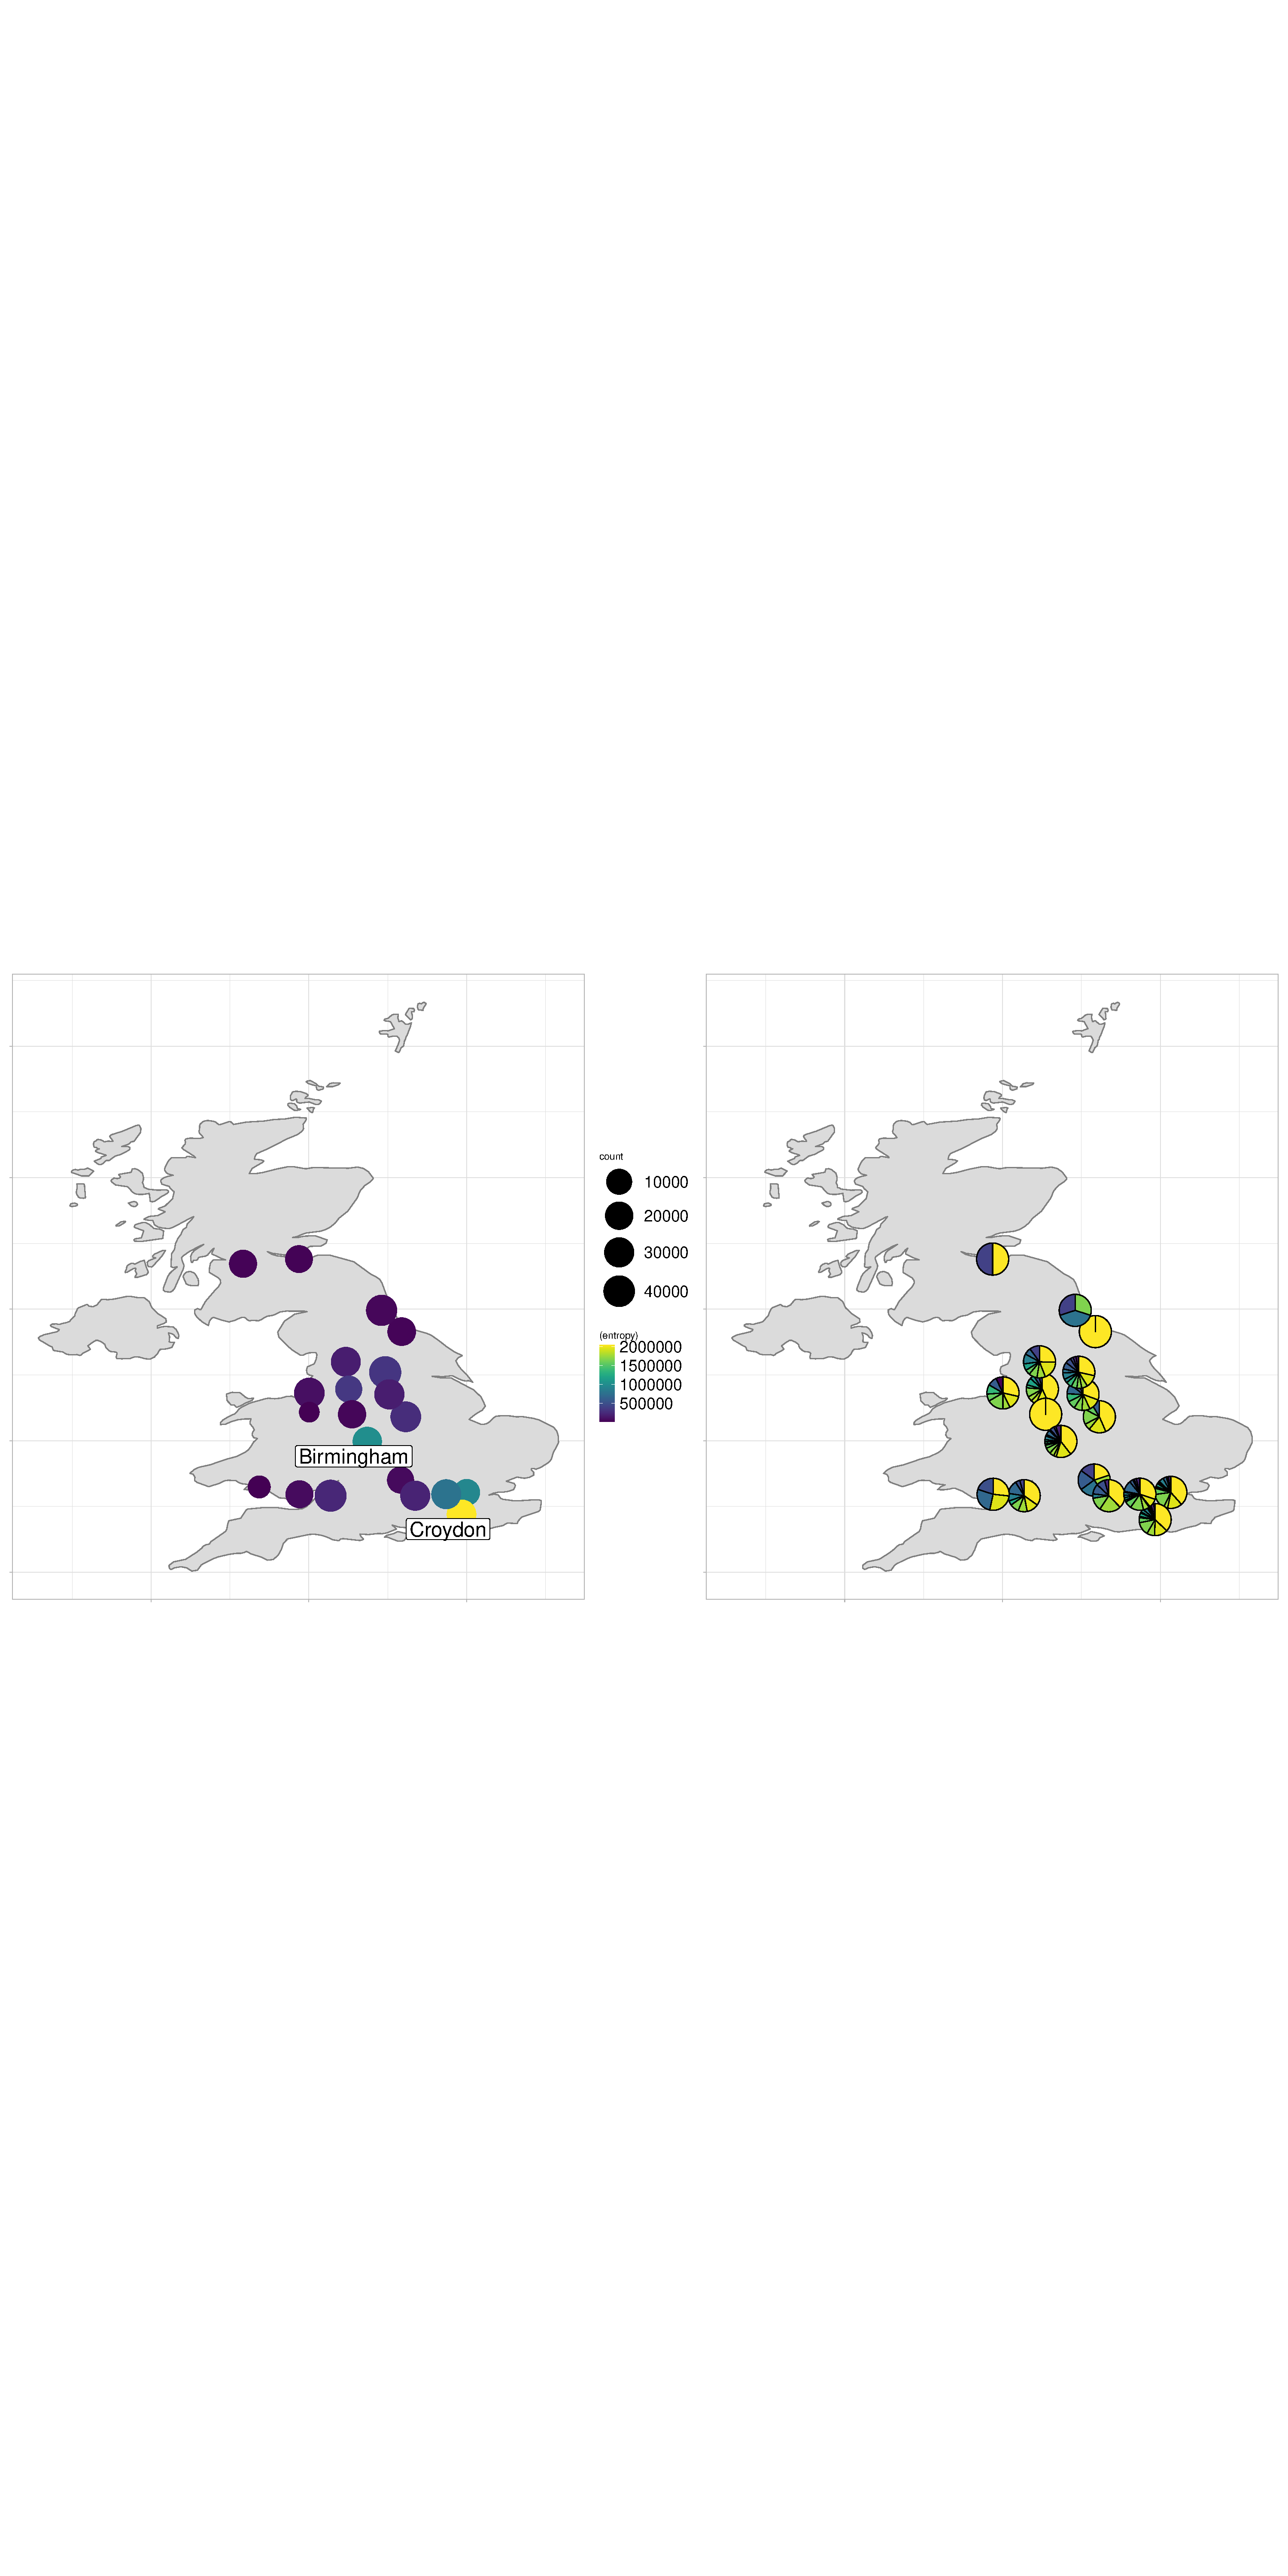
\includegraphics[width=1.0\textwidth]{../images/chapter3/SF_props_pie_chart.pdf}
    \vspace{-1mm}
    \caption{Distribution of ethnicities across different testing centres. Each pie corresponds to a U.K. Biobank testing centre, with each section of the each pie corresponding to a different ethnicity. Jitter added to points to avoid overlapping. }
    \label{fig:SF_props_pie_chart_entropy_map}
\end{sidewaysfigure}

\subsection{Patterns of African ancestry across the U.K.}

I also had access to the birth-date of each U.K. Biobank participant. Therefore, it is possible to calculate the increase of the ancestry of a particular ethnic group over time based on birth-year (Fig.  \ref{fig:rollingaverage_time_Buganda_ancestry}). I took all U.K. Biobank individuals with more than 50\% African ancestry and split them into 50 bins according to their birth date. Using a rolling window in the \texttt{rollyapply} function from the \texttt{zoo} R library, I calculated the mean proportion of all ancestries across ancestry for each bin. Fig \ref{fig:rollingaverage_time_Buganda_ancestry} shows the increase of Buganda ancestry over time. 

\begin{figure}[htp]
    \centering
    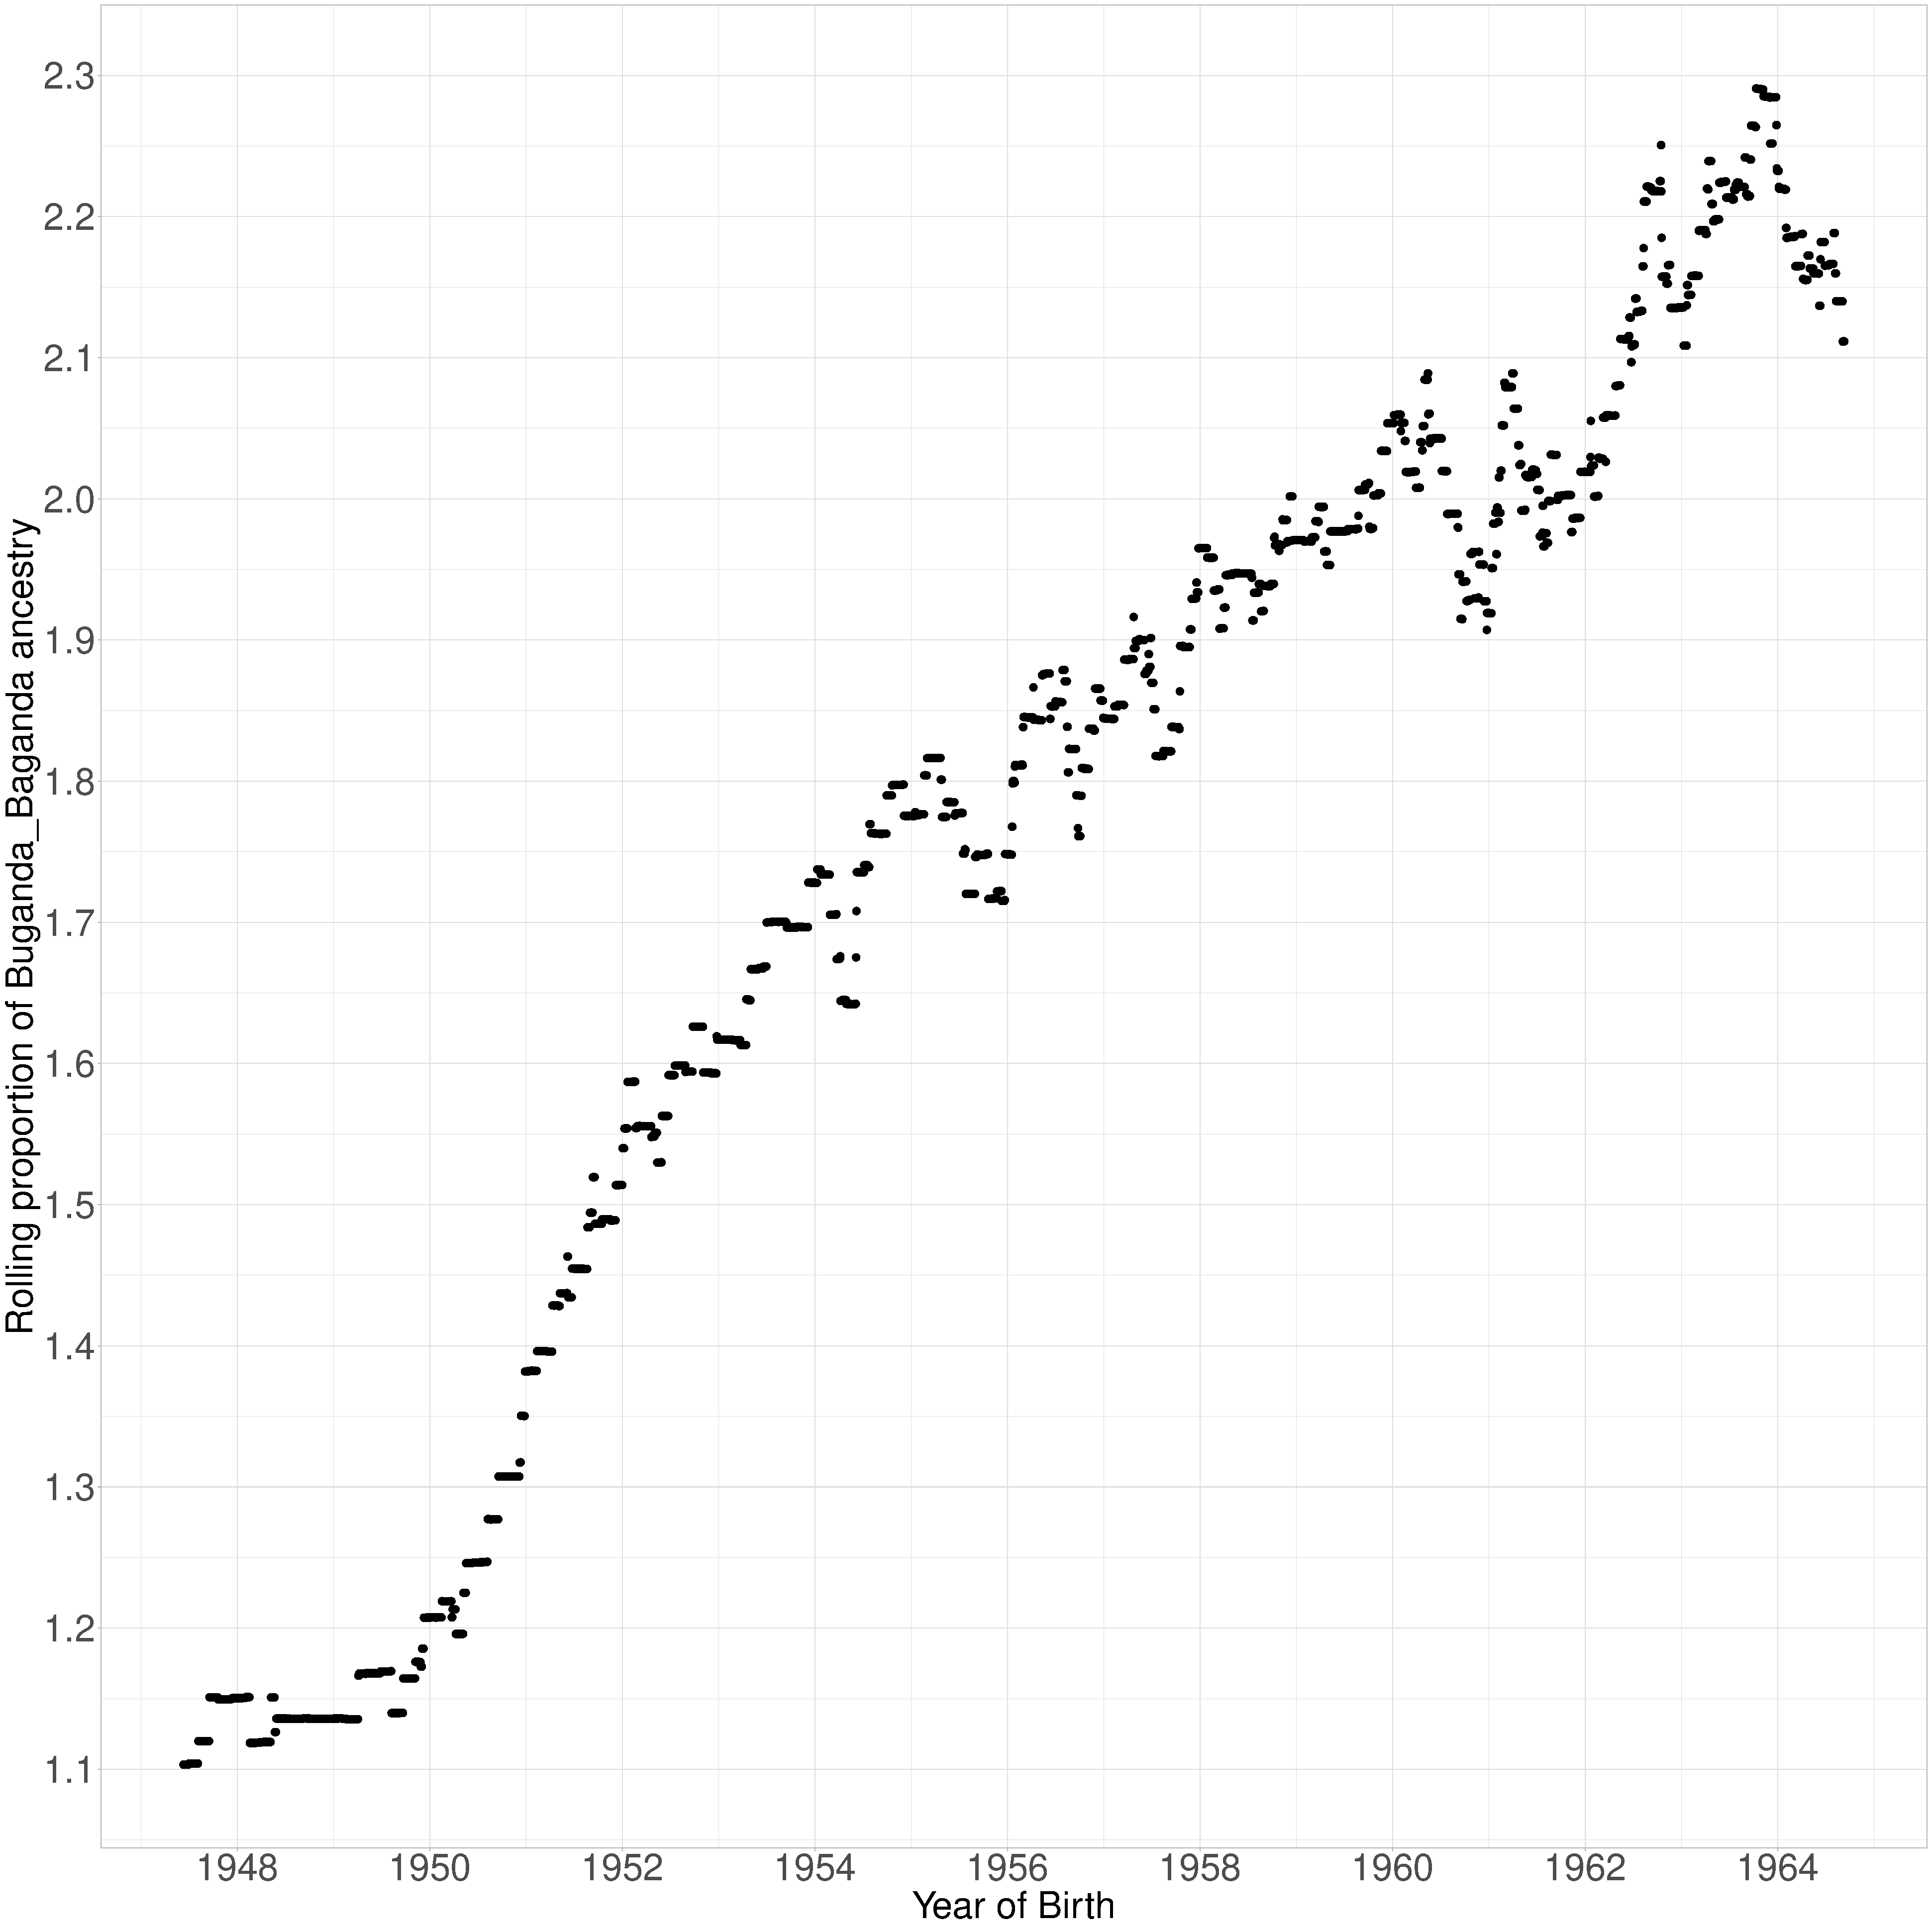
\includegraphics[width=1.0\textwidth]{../images/chapter3/rollingaverage_time_Buganda_ancestry.pdf}
    \caption{Increase in the mean proportion of Buganda ancestry between 1948 and 1965. An overlapping sliding window was applied to SOURCEFIND ancestry proportions and mean proportion of Buganda ancestry for each window plotted against the mean birth-date of individuals in that bin.}
    \label{fig:rollingaverage_time_Buganda_ancestry}
\end{figure}

We can observe roughly a doubling of the mean proportion of  Buganda\_Baganda ancestry between 1950 and 1964. In 1972, then president Idi Amin expelled roughly 60,000 Ugandans to the U.K. Therefore, this increase may tentatively correspond to an increase in the number of individuals between the ages of 7-22 arriving in the U.K. during these dates. 

\section{Summary of Results and Discussion} 

The aim of this chapter was twofold; firstly, to determine whether using less dense non-imputed or more dense imputed SNPs is preferable when combining genotype data from multiple chips. Secondly, I wanted to explore the diversity of African ancestry in the U.K. Biobank and its relation to population history.  

I also showed that, in individuals with recent African ancestry, there is enough linkage information across 70,000 genome-wide SNPs to recover a substantial amount of useful haplotype information and accurately predict the birth country of a sample. Further, I found that using the particular imputation strategy I employed, namely imputing missing genotypes in genotype arrays after merging datasets, significantly reduces the power to assign African individuals to the correct population. This imputation strategy also introduces a degree of bias, in that donor groups donate more to populations present in the reference panel when using imputed data relative to non-imputed data. Future work should explore the downstream effects of such bias when e.g. estimating ancestry proportions of inferring genetic clusters. 

West African ancestry was the most common across samples with recent African ancestry, with ancestry from ethnic groups from Nigeria and Ghana being especially prevalent. In particular, individuals had substantially more ancestry from Yoruba than any other ethnicity. I did not find evidence for structure in how African ancestry was distributed across the U.K., based on the testing centre that participants registered at. 

Future work on using Biobanks to explore population structure and history could focus on two points.
Ideally, I would liked to have painted the entire U.K. Biobank dataset using the Human Origins dataset as a reference panel, rather than restricting analysis to individuals with 50\% recent African ancestry. This would have allowed me to analyse a substantially higher amount of African haplotypes across the entire dataset and this give a more complete extent of African ancestry in the U.K. Thus, the development of efficient methods, likely based on the PBWT, which allow for Biobank-scale datasets to be painted by large reference panels would accelerate research into ethnic minority ancestries. 

Secondly, larger reference panels of worldwide populations and more ethnic groups will allow for a more detailed characterisation of genetic variation.  Similarly, including details on ethnic identity in Biobank projects would improve the resolution at which analysis could be carried out.  


